%\documentclass[a4paper,11pt]{article}
\documentclass{article}
%%%%%%%%%%%%%%%%%%%%%%%%%%%%%%%%%%%%%%%%%%%%%%%%%%%%%%%%%%%%%%%%%%%%%%%%%%%%%%%%%%%%%%%%%%%%%%%%%%%%%%%%%%%%%%%%%%%%%%%%%%$•$%%
\usepackage{graphics,graphicx}
\usepackage{subcaption}
\usepackage{amsmath,amssymb,graphics,graphicx}
\usepackage[usenames,dvipsnames]{color}
\usepackage[spanish]{babel}
\renewcommand{\spanishtablename}{Tabla}
\renewcommand{\spanishfigurename}{Figura}

\graphicspath{{Images/}}
\usepackage{natbib}

\bibpunct{(}{)}{;}{a}{,}{,}

\textheight 24cm \textwidth 17cm \topmargin-2cm
%% \evensidemargin   -0.25cm
\oddsidemargin-0.2cm
%\pagestyle{empty}
\renewcommand{\baselinestretch}{1}

\begin{document}

%\title{}

%\address{}
\begin{titlepage}
	\centering
	{\bfseries\LARGE Universidad Polit\'ecnica de Madrid \par}
	\vspace{1cm}
	{\scshape\Large M\'aster Universitario en Inteligencia Artificial \par}
	\vspace{3cm}
	{\scshape\Huge Pr\'actica 1: FIFA Players Classification \par}
	\vspace{3cm}
	{\Large Asignatura: Artificial neural networks and deep learning \par}
	\vfill
	{\Large Autores: \par}
	{\Large Juan José Flores Arellano \par
	 		Borja Reinoso Hidalgo \par 
	 		Daniel Carmona Pedrajas \par}
	\vfill
	{\Large Correos: \par}
	{\Large jj.flores.arellano@alumnos.upm.es \par
			borja.reinoso@alumnos.ump.es \par 
	 		daniel.carmonap@alumnos.upm.es \par}	
	\vfill
	{\Large 16 Diciembre 2022 \par}
\end{titlepage}

\tableofcontents
	\section{Introducci\'on}
	\label{intro}
		Este proyecto tiene como objetivo diseñar una red neuronal artificial para resolver un problema de clasificación supervisada de jugadores del videojuego FIFA 19. Para ello se hará uso de las técnicas y herramientas aprendidas en la clase de “Redes de neuronas artificiales y deep learning”.\\

	Se hará uso del lenguaje de programación Python 3 junto a las librerías Tensorflow 2 y Keras. Los entornos utilizados serán: Jupyter notebook en local y Google Colab.\\

	El dataset a utilizar es {}. Este dataset contiene 18.207 instancias con 89 atributos cada una. Tras un preprocesado se han reducido tanto las instancias como los atributos a utilizar, 16.122 instancias con 17 atributos cada una. Los atributos están relacionados con la habilidad de cada jugador en ciertas facetas relacionadas con el fútbol: Crossing, Heading Accuracy, Pase Corto, Voleas, Regate, Curva, Precisión de Tiro Libre, Pase Largo, Control del Balón, Reacción, Potencia de Tiro, Resistencia, Tiros lejanos, Agresividad, Posicionamiento, Visión y Compostura.\\

	Para etiquetar las clases se ha hecho una media de los atributos de los jugadores y se ha repartido de la siguiente manera: 
	\begin{enumerate}
		\item Poor para medias entre [46,62]
    	\item Intermediate para medias entre [63,66]
    	\item Good para medias entre [67,71]
    	\item Excellent para medias entre [72,94]
	\end{enumerate}
	
	\subsection{Estructura}
		La investigaci\'on se divide en dos fases:
		\begin{itemize}
			\item Familiarizaci\'on con hiperpar\'ametros y t\'ecnicas de regularizaci\'on.
			\item Optimizaci\'on sistem\'atica de hiperpar\'ametros
		\end{itemize}
		
		En ambas partes realizaremos cambios at\'omicos para comprobar el efecto de los mismos en el modelo, pero en la primera fase trabajamos de una forma reactiva, solucionando los problemas que nos surgen para comprender el impacto de cada cambio que hacemos. Una vez interiorizados estos efectos pasamos a comprobar distintos valores para cada hiperpar\'ametro para quedarnos con el mejor, fijarlo en la configuraci\'on y pasar al siguiente.\\
		
		Por \'ultimo, presentaremos nuestras conclusiones.

\section{Fase 1: Cambios reactivos}
	Como hemos comentado, en esta fase iremos realizando peque\~nos cambios, observando c\'omo afectan a los resultados del modelo y al proceso de entrenamiento.
	\subsection{Arquitectura 1: Feed Forward Neural Network}
	\label{d-s-a1}
		La primera arquitectura que usaremos es tan simple como:
		\begin{enumerate}
			\item Capa densa con 512 neuronas.
		\end{enumerate}
		\subsubsection{Experimento 1: Configuraci\'on base arbitraria}
		\label{d-s-a1-e1}
			Usamos la siguiente configuraci\'on:
			\begin{table}[!h]
				\begin{center}
					\begin{tabular}{| c | c | c | c | c | c | c |}
						\textbf{Epochs} & \textbf{Learning rate} & \textbf{Batch size} & \textbf{Activation} & \textbf{Loss} & \textbf{Optimizer} & \textbf{Regularization} \\ \hline
						100 & 0.1 & 512 & ReLU & Categorical Crossentropy & SGD & None
					\end{tabular}
					\caption{Hiperpar\'ametros para el Experimento 1 de la Arquitectura 1}
					\label{tab:hip-d-a1-e1}
				\end{center}
			\end{table}
		
			Y entrenamos 5 veces para obtener los siguientes resultados:
			\begin{table}[!h]
				\begin{center}
					\begin{tabular}{ c | c | c | c | c | c |}
						\ & \textbf{Train accuracy (\%)} & \textbf{Validation accuracy (\%)} & \textbf{Bias (\%)} & \textbf{Variance (\%)} & \textbf{Training time (s)} \\ \hline
						\textbf{Mean} & 79.38 & 77.94 & 15.61 & 1.44 & 14\\ \hline
						\textbf{Std} & 0.05 & 0.14 & 0.05 & 0.19 & 0 \\ \hline
					\end{tabular}
					\caption{Resultados del Experimento 1 de la Arquitectura 1}
					\label{tab:res-d-a1-e1}
				\end{center}
			\end{table}
		
			Tener un \textit{bias} alto y una \textit{variance} baja significa que hay margen de mejora antes de llegar al \textit{overfitting} y hay varias posibilidades para conseguir una mejor \textit{accuracy}: a\~nadir m\'as neuronas, entrenar con m\'as \textit{epochs}, ...
		
		\subsubsection{Experimento 2: Aumentamos \textit{epochs}}
		\label{d-s-a1-e2}
			Tras el experimento anterior, nos decantamos por entrenar el modelo durante m\'as \textit{epochs} para reducir el \textit{bias} usando la misma configuraci\'on.\\
			\begin{table}[!h]
				\begin{center}
					\begin{tabular}{| c | c | c | c | c | c | c |}
						\textbf{Epochs} & \textbf{Learning rate} & \textbf{Batch size} & \textbf{Activation} & \textbf{Loss} & \textbf{Optimizer} & \textbf{Regularization} \\ \hline
						\textbf{1000} & 0.1 & 512 & ReLU & Categorical Crossentropy & SGD & None
					\end{tabular}
					\caption{Hiperpar\'ametros para el Experimento 2 de la Arquitectura 1}
					\label{tab:hip-d-a1-e2}
				\end{center}
			\end{table}
			
			Tras 5 entrenamientos obtenemos los siguientes resultados:
			\begin{table}[!h]
				\begin{center}
					\begin{tabular}{ c | c | c | c | c | c |}
						\ & \textbf{Train accuracy (\%)} & \textbf{Validation accuracy (\%)} & \textbf{Bias (\%)} & \textbf{Variance (\%)} & \textbf{Training time (s)} \\ \hline
						\textbf{Mean} & 84.02 & 81.5 & 10.97 & 2.47 & 199\\ \hline
						\textbf{Std} & 0.03 & 0.17 & 0.03 & 0.18 & 8.8 \\ \hline
					\end{tabular}
					\caption{Resultados del Experimento 2 de la Arquitectura 1}
					\label{tab:res-d-a1-e2}
				\end{center}
			\end{table}
			Con respecto al experimento anterior hemos aumentado el \textit{accuracy} tanto en el entrenamiento como en validaci\'on, reduciendo as\'i el \textit{bias} del modelo en un 5\% aunque ha aumentado ligeramente el \textit{variance}. Como es l\'ogico el tiempo de entrenamiento ha crecido, aunque no de forma lineal.\\
			\begin{figure}[!h]
				\begin{center}
					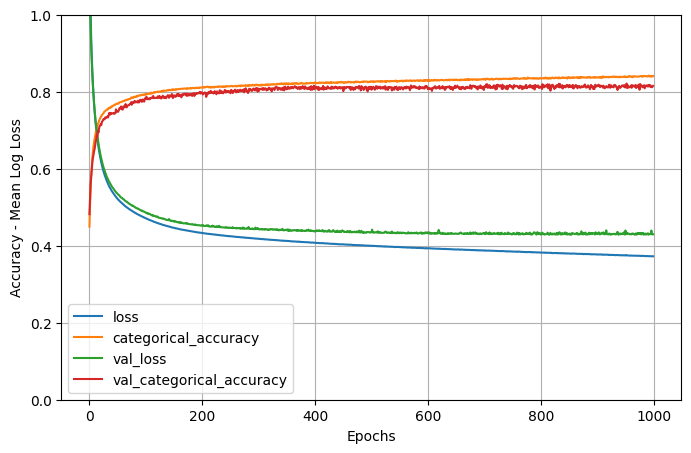
\includegraphics[scale=0.5]{d-tr-a1-e2.png}		
					\caption{Entrenamiento durante el Experimento 2 de la Arquitectura 1}	
					\label{d-tr-a1-e2}
				\end{center}
			\end{figure}
			En la figura \ref{d-tr-a1-e2} vemos que a partir del epoch 400 no hay una mejora en \textit{accuracy} para el conjunto de validaci\'on aunque s\'i para el conjunto de entrenamiento lo que nos indica que un n\'umero de \textit{epochs} tan elevado como el que hemos usado en este experimento con esta arquitectura y configuraci\'on conduce a un \textit{overfitting} del modelo, aunque por el momento no es excesivo como nos indica la \textit{variance}.
			
		\subsubsection{Experimento 3: Cambiamos a \textit{tanh} y reducimos \textit{epochs}}
		\label{d-s-a1-e3}
			Para este experimento decidimos reducir las \textit{epochs} ya que como hemos visto en el experimento anterior, no hay una mejora significativa en validaci\'on con m\'as epochs.\\
			Adem\'as de esto, cambiaremos la funci\'on de activaci\'on a \textit{tanh}. Hasta el momento hemos usado \textit{ReLU} pero no hay raz\'on para usarla para esta arquitectura porque resuelve el problema del \textit{vanishing gradient} que se da en arquitecturas profundas.\\
			La configuraci\'on que usamos para el experimento 3 es:
			\begin{table}[!h]
				\begin{center}
					\begin{tabular}{| c | c | c | c | c | c | c |}
						\textbf{Epochs} & \textbf{Learning rate} & \textbf{Batch size} & \textbf{Activation} & \textbf{Loss} & \textbf{Optimizer} & \textbf{Regularization} \\ \hline
						\textbf{400} & 0.1 & 512 & \textbf{tanh} & Categorical Crossentropy & SGD & None
					\end{tabular}
					\caption{Hiperpar\'ametros para el Experimento 3 de la Arquitectura 1}
					\label{tab:hip-d-a1-e3}
				\end{center}
			\end{table}
			
			Tras 5 entrenamientos obtenemos los siguientes resultados:
			\begin{table}[!h]
				\begin{center}
					\begin{tabular}{ c | c | c | c | c | c |}
						\ & \textbf{Train accuracy (\%)} & \textbf{Validation accuracy (\%)} & \textbf{Bias (\%)} & \textbf{Variance (\%)} & \textbf{Training time (s)} \\ \hline
						\textbf{Mean} & 79.58 & 78.3 & 15.41 & 1.28 & 72\\ \hline
						\textbf{Std} & 0.2 & 0.51 & 0.22 & 0.33 & 3.27 \\ \hline
					\end{tabular}
					\caption{Resultados del Experimento 3 de la Arquitectura 1}
					\label{tab:res-d-a1-e3}
				\end{center}
			\end{table}
			
			Con esta configuraci\'on el modelo ha vuelto a aumentar el \textit{bias} y obtenemos unos resultados pr\'acticamente id\'enticos al experimento uno con la funci\'on de activaci\'on \textit{ReLU} aunque con m\'as epochs. Parece que con la funci\'on \textit{tanh}, el modelo se queda atrapado en m\'inimos globales como podemos apreciar en la figura \ref{d-tr-a1-e3} y necesita m\'as epochs para escapar de ellos.\\
			
			\begin{figure}[!h]
				\begin{center}
					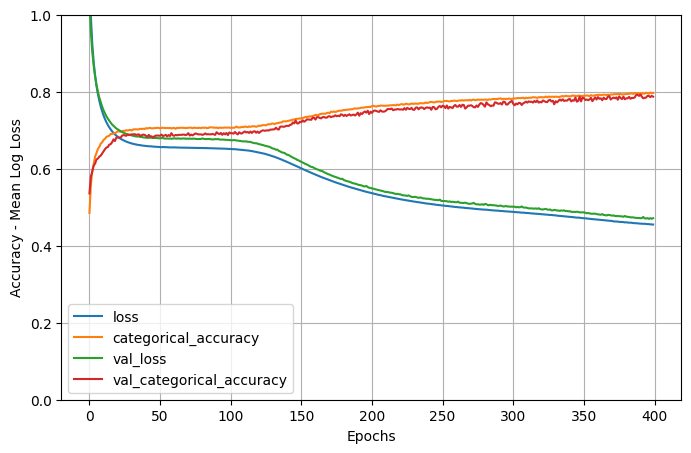
\includegraphics[scale=0.5]{d-tr-a1-e3.png}		
					\caption{Entrenamiento durante el Experimento 3 de la Arquitectura 1}	
					\label{d-tr-a1-e3}
				\end{center}
			\end{figure}
			
			Tambi\'en observamos que no ha habido overfitting hasta la epoch 400, al contrario de lo que hab\'iamos supuesto al inicio de este experimento.
			
		\subsubsection{Experimento 4: Aumentamos \textit{epochs}}
		\label{d-s-a1-e4}
			El objetivo de este experimento es comprobar cu\'antas \textit{epochs} podemos realizar antes de que el modelo comience a dirigirse hacia un \textit{overfitting} por lo que la configuraci\'on es la misma que en la ejecuci\'on anterior, excepto que volvemos a incrementar las epochs a 1000:
			\begin{table}[!h]
				\begin{center}
					\begin{tabular}{| c | c | c | c | c | c | c |}
						\textbf{Epochs} & \textbf{Learning rate} & \textbf{Batch size} & \textbf{Activation} & \textbf{Loss} & \textbf{Optimizer} & \textbf{Regularization} \\ \hline
						\textbf{1000} & 0.1 & 512 & tanh & Categorical Crossentropy & SGD & None
					\end{tabular}
					\caption{Hiperpar\'ametros para el Experimento 4 de la Arquitectura 1}
					\label{tab:hip-d-a1-e4}
				\end{center}
			\end{table}
			
			Tras 5 entrenamientos obtenemos los siguientes resultados:
			\begin{table}[!h]
				\begin{center}
					\begin{tabular}{ c | c | c | c | c | c |}
						\ & \textbf{Train accuracy (\%)} & \textbf{Validation accuracy (\%)} & \textbf{Bias (\%)} & \textbf{Variance (\%)} & \textbf{Training time (s)} \\ \hline
						\textbf{Mean} & 81.17 & 80.23 & 13.82 & 0.94 & 189\\ \hline
						\textbf{Std} & 0.14 & 0.62 & 0.14 & 0.53 & 2.3 \\ \hline
					\end{tabular}
					\caption{Resultados del Experimento 4 de la Arquitectura 1}
					\label{tab:res-d-a1-e4}
				\end{center}
			\end{table}
			
			\begin{figure}[!h]
				\begin{center}
					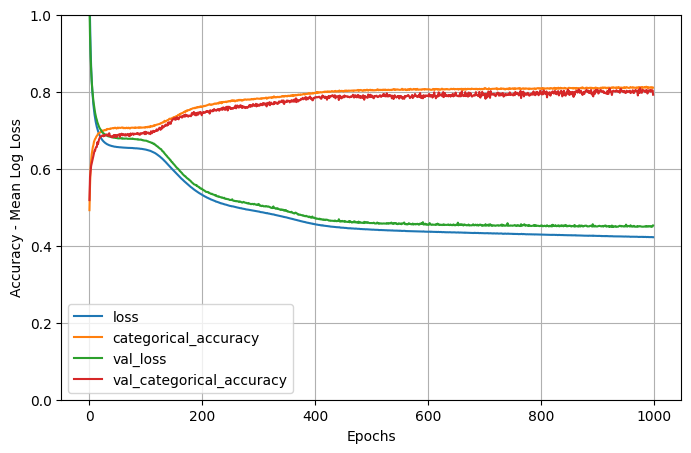
\includegraphics[scale=0.5]{d-tr-a1-e4.png}		
					\caption{Entrenamiento durante el Experimento 4 de la Arquitectura 1}	
					\label{d-tr-a1-e4}
				\end{center}
			\end{figure}
			
			Aunque hemos doblado las \textit{epochs} con respecto al experimento 3, la mejora ha sido de apenas un 2\% en \textit{accuracy}. Por otra parte, como se muestra en la figura \ref{d-tr-a1-e4}, el modelo no ha llegado al punto de \textit{overfitting} aun habiendo usado un n\'umero tan alto de epochs.\\
			Esto quiere decir que todav\'ia hay margen de mejora si seguimos entrenando con m\'as epochs aunque llevar\'ia mucho tiempo porque el aprendizaje es lento.\\
			
		\subsubsection{Experimento 5: Reducimos \textit{batch size}}
		\label{d-s-a1-e5}
			Como se necesitar\'ia aumentar exponencialmente el n\'umero de \textit{epochs} para conseguir una mejora en el \textit{accuracy}, decidimos reducir el \textit{batch size} y comprobar si de esta forma el modelo consigue mejores resultados.
			\begin{table}[!h]
				\begin{center}
					\begin{tabular}{| c | c | c | c | c | c | c |}
						\textbf{Epochs} & \textbf{Learning rate} & \textbf{Batch size} & \textbf{Activation} & \textbf{Loss} & \textbf{Optimizer} & \textbf{Regularization} \\ \hline
						1000 & 0.1 & \textbf{128} & tanh & Categorical Crossentropy & SGD & None
					\end{tabular}
					\caption{Hiperpar\'ametros para el Experimento 5 de la Arquitectura 1}
					\label{tab:hip-d-a1-e5}
				\end{center}
			\end{table}
			
			Tras 5 entrenamientos obtenemos los siguientes resultados:\\
			\begin{table}[!h]
				\begin{center}
					\begin{tabular}{ c | c | c | c | c | c |}
						\ & \textbf{Train accuracy (\%)} & \textbf{Validation accuracy (\%)} & \textbf{Bias (\%)} & \textbf{Variance (\%)} & \textbf{Training time (s)} \\ \hline
						\textbf{Mean} & 82.92 & 80.84 & 12.07 & 2.08 & 517.2\\ \hline
						\textbf{Std} & 0.19 & 0.29 & 0.19 & 0.28 & 25.61 \\ \hline
					\end{tabular}
					\caption{Resultados del Experimento 4 de la Arquitectura 1}
					\label{tab:res-d-a1-e5}
				\end{center}
			\end{table}
			Como vemos en la tabla \ref{tab:res-d-a1-e5} no conseguimos mejorar de forma significativa el \textit{accuracy}. Aumentar el \textit{batch size} ha incrementado exponencialmente el tiempo de entrenamiento por lo que no merece la pena reducir el \textit{batch size} en este caso. Lo que hemos conseguido reduciendo el \textit{batch size} ha sido que el modelo escape r\'apidamente del primer m\'inimo local con el que se topa como vemos en la figura \ref{d-tr-a1-e5} as\'i que concluimos que con esta t\'ecnica podemos obtener un resultado aceptable en menor tiempo.
			\begin{figure}[!h]
				\begin{center}
					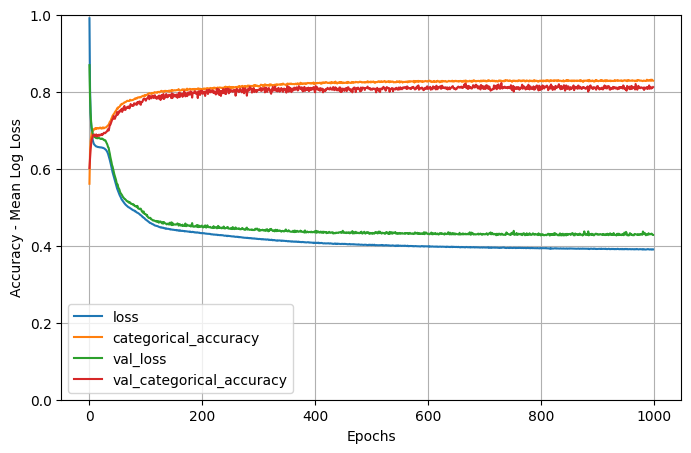
\includegraphics[scale=0.5]{d-tr-a1-e5.png}		
					\caption{Entrenamiento durante el Experimento 5 de la Arquitectura 1}	
					\label{d-tr-a1-e5}
				\end{center}
			\end{figure}
			
		\subsubsection{Conclusiones de la Arquitectura 1}
		\label{d-cl-a1}
			\begin{itemize}
				\item \textit{ReLU} llega a un estado de \textit{overfitting} con menos \textit{epochs} que \textit{tanh}
				\item \textit{tanh} tiene un proceso de aprendizaje m\'as lento que \textit{ReLU}
				\item Reducir el \textit{batch size} implica llegar a un \'optimo de forma m\'as r\'apida con \textit{tanh}.
			\end{itemize}
			
	\subsection{Arquitectura 2: Deep Feed Forward Neural Network}
	\label{d-s-a2}
		Hemos visto que con la arquitectura anterior obtenemos un \textit{accuracy} m\'aximo de un 84\% a partir de donde el aprendizaje es lento y llegamos a un \textit{overfitting} con las t\'ecnicas utilizadas. Es por esto que decidimos usar una Deep Feed Forward Neural Network para intentar reducir el \textit{bias} del modelo.\\
		La arquitectura que utilizaremos para la nueva serie de experimento ser\'a:
		
		\begin{enumerate}
			\item Capa densa de 128 neuronas
			\item Capa densa de 64 neuronas
			\item Capa densa de 32 neuronas
		\end{enumerate}
		
		\subsubsection{Experimento 1: Comparaci\'on con arquitectura 1}
		\label{d-s-a2-e1}
			En este experimento utilizaremos la misma configuraci\'on que en el experimento anterior:
			\begin{table}[!h]
				\begin{center}
					\begin{tabular}{| c | c | c | c | c | c | c |}
						\textbf{Epochs} & \textbf{Learning rate} & \textbf{Batch size} & \textbf{Activation} & \textbf{Loss} & \textbf{Optimizer} & \textbf{Regularization} \\ \hline
						1000 & 0.1 & 128 & tanh & Categorical Crossentropy & SGD & None
					\end{tabular}
					\caption{Hiperpar\'ametros para el Experimento 1 de la Arquitectura 2}
					\label{tab:hip-d-a2-e1}
				\end{center}
			\end{table}
			
			Tras 5 entrenamientos obtenemos los siguientes resultados:
			
			\begin{table}[!h]
				\begin{center}
					\begin{tabular}{ c | c | c | c | c | c |}
						\ & \textbf{Train accuracy (\%)} & \textbf{Validation accuracy (\%)} & \textbf{Bias (\%)} & \textbf{Variance (\%)} & \textbf{Training time (s)} \\ \hline
						\textbf{Mean} & 99.89 & 74.97 & -4.89 & 24.91 & 578\\ \hline
						\textbf{Std} & 0.04 & 0.26 & 0.04 & 0.26 & 4.54 \\ \hline
					\end{tabular}
					\caption{Resultados del Experimento 1 de la Arquitectura 2}
					\label{tab:res-d-a2-e1}
				\end{center}
			\end{table}
			
			Hemos obtenido un modelo con un \textit{overfitting} muy alto, tan alto que ha cometido menos error que un humano y por eso el \textit{bias} es negativo. Podemos ver el \textit{overfitting} reflejado en el \textit{variance} de un 25\% de la tabla \ref{tab:res-d-a2-e1} y la evoluci\'on del \textit{validation categorical accuracy} en la figura \ref{d-tr-a2-e1} que empeora a lo largo del entrenamiento.
			
			\begin{figure}[!h]
				\begin{center}
					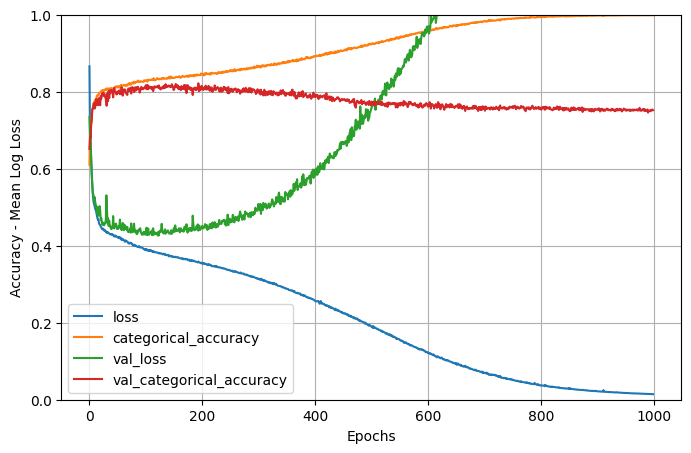
\includegraphics[scale=0.5]{d-tr-a2-e1.png}		
					\caption{Entrenamiento durante el Experimento 1 de la Arquitectura 2}	
					\label{d-tr-a2-e1}
				\end{center}
			\end{figure}
			
			\newpage
			
			
		\subsubsection{Experimento 2: Reducimos \textit{epochs} y utilizamos regularizaci\'on}
		\label{d-s-a2-e2}
			Una de las t\'ecnicas que podemos utilizar para reducir el \textit{variance} es usar regularizaci\'on para controlar que los pesos de las neuronas no se hagan demasiado grande. Adem\'as para ahorrar algo de tiempo tambi\'en reduciremos las epochs. La configuraci\'on para este experimento queda reflejada en la tabla \ref{tab:hip-d-a2-e2}.
			\begin{table}[!h]
				\begin{center}
					\begin{tabular}{| c | c | c | c | c | c | c |}
						\textbf{Epochs} & \textbf{Learning rate} & \textbf{Batch size} & \textbf{Activation} & \textbf{Loss} & \textbf{Optimizer} & \textbf{Regularization} \\ \hline
						\textbf{400} & 0.1 & 128 & tanh & Categorical Crossentropy & SGD & \textbf{l2 0.001}
					\end{tabular}
					\caption{Hiperpar\'ametros para el Experimento 2 de la Arquitectura 2}
					\label{tab:hip-d-a2-e2}
				\end{center}
			\end{table}
			
			Tras 5 entrenamientos obtenemos los siguientes resultados:
			
			\begin{table}[!h]
				\begin{center}
					\begin{tabular}{ c | c | c | c | c | c |}
						\ & \textbf{Train accuracy (\%)} & \textbf{Validation accuracy (\%)} & \textbf{Bias (\%)} & \textbf{Variance (\%)} & \textbf{Training time (s)} \\ \hline
						\textbf{Mean} & 81.19 & 79.91 & 13.8 & 1.28 & 249\\ \hline
						\textbf{Std} & 0.2 & 0.95 & 0.2 & 0.92 & 3.29 \\ \hline
					\end{tabular}
					\caption{Resultados del Experimento 2 de la Arquitectura 2}
					\label{tab:res-d-a2-e2}
				\end{center}
			\end{table}
			
			Como se observa en la tabla \ref{tab:res-d-a2-e2}, hemos conseguido reducir el \textit{variance} un 24\% simplemente usando regularizaci\'on, ahora bien, en cuanto a \textit{accuracy} seguimos sin conseguir una mejora significativa.
			
			\begin{figure}[!h]
				\begin{center}
					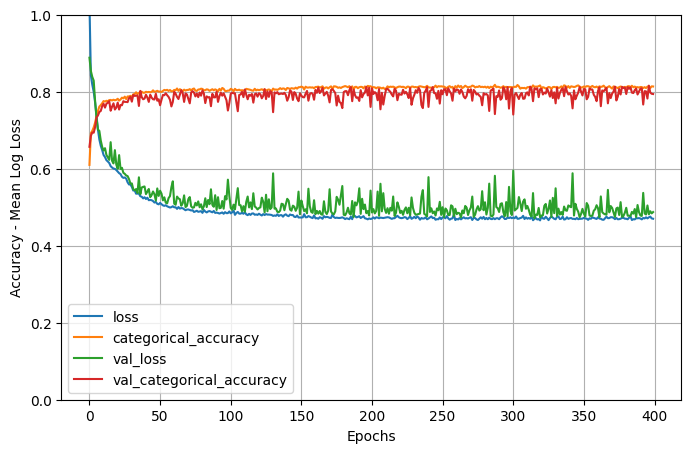
\includegraphics[scale=0.5]{d-tr-a2-e2.png}		
					\caption{Entrenamiento durante el Experimento 2 de la Arquitectura 2}	
					\label{d-tr-a2-e2}
				\end{center}
			\end{figure}
			
			En la figura \ref{d-tr-a2-e2} se aprecia ruido en las m\'etricas del conjunto de validaci\'on, esto es una consecuencia de la regularizaci\'on, sin ella ese ruido se descontrolar\'ia y llegar\'iamos al \textit{overfitting} como en el experimento anterior.
			
			
		\subsubsection{Experimento 3: Cambiamos el optimizador}
		\label{d-s-a2-e3}
			En este experimento vamos a comprobar si con un optimizador distinto podemos obtener mejor \textit{accuracy} sin llegar al \textit{overfitting}, para ello utilizaremos ADAM. La configuraci\'on es la siguiente:
			
			\begin{table}[!h]
				\begin{center}
					\begin{tabular}{| c | c | c | c | c | c | c |}
						\textbf{Epochs} & \textbf{Learning rate} & \textbf{Batch size} & \textbf{Activation} & \textbf{Loss} & \textbf{Optimizer} & \textbf{Regularization} \\ \hline
						400 & 0.1 & 128 & tanh & Categorical Crossentropy & \textbf{ADAM} & l2 0.001
					\end{tabular}
					\caption{Hiperpar\'ametros para el Experimento 3 de la Arquitectura 2}
					\label{tab:hip-d-a2-e3}
				\end{center}
			\end{table}
			
			\newpage
			Tras 5 entrenamientos obtenemos los siguientes resultados:
			
			\begin{table}[!h]
				\begin{center}
					\begin{tabular}{ c | c | c | c | c | c |}
						\ & \textbf{Train accuracy (\%)} & \textbf{Validation accuracy (\%)} & \textbf{Bias (\%)} & \textbf{Variance (\%)} & \textbf{Training time (s)} \\ \hline
						\textbf{Mean} & 25.34 & 26.25 & 69.65 & -0.91 & 266.8 \\ \hline
						\textbf{Std} & 0.29 & 2.61 & 0.29 & 2.44 & 4.81 \\ \hline
					\end{tabular}
					\caption{Resultados del Experimento 3 de la Arquitectura 2}
					\label{tab:res-d-a2-e3}
				\end{center}
			\end{table}
			
			Como vemos en la tabla resultados son los peores obtenidos hasta el momento y con mucha diferencia, apenas hemos conseguido un 25\% de \textit{accuracy}. Analizando la figura \ref{d-tr-a2-e3}, el modelo se queda estancado en un m\'inimo local muy temprano en el entrenamiento.
			\begin{figure}[!h]
				\begin{center}
					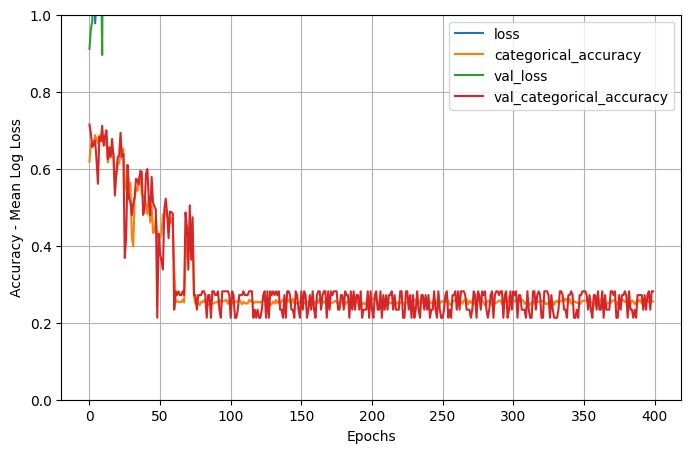
\includegraphics[scale=0.5]{d-tr-a2-e3.png}		
					\caption{Entrenamiento durante el Experimento 4 de la Arquitectura 2}	
					\label{d-tr-a2-e3}
				\end{center}
			\end{figure}
			
			Observando la matriz de confusi\'on confirmamos nuestra teor\'ia, clasifica todos los jugadores en la misma clase.
			\begin{figure}[!h]
				\begin{center}
					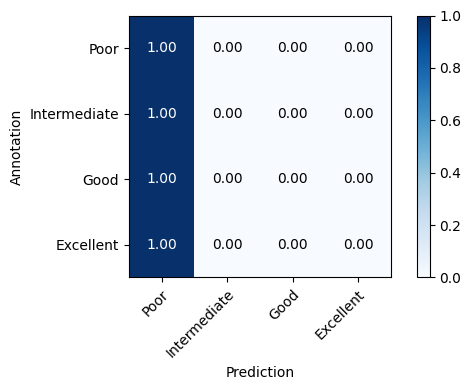
\includegraphics[scale=0.7]{d-cm-a2-e3.png}		
					\caption{Matriz de confusi\'on en el Experimento 3 de la Arquitectura 2}	
					\label{d-cm-a2-e3}
				\end{center}
			\end{figure}
			
			Esto puede deberse a que no estamos usando correctamente el optimizador ADAM.
			
			
		\subsubsection{Experimento 4: Ajustamos el optimizador ADAM}
		\label{d-s-a2-e4}
			Consultando el art\'iculo en el que se present\'o ADAM (\textit{Adam: A Method for Stochastic Optimization}, (2015), D. Kingma y J. Ba), vemos que este optimizador es una combinaci\'on entre AdaGrad y RMSProp y que tiene unos par\'ametros que controlan el ratio de decrecimiento de los momentos (beta1=0.9 y beta2=0.999) que no hemos definido en el experimento anterior. Adem\'as de esto, los autores sugieren usar un \textit{learning rate} m\'as bajo del que estamos usando.\\
			
			La configuraci\'on queda as\'i:
			\begin{table}[!h]
				\begin{center}
					\begin{tabular}{| c | c | c | c | c | c | c |}
						\textbf{Epochs} & \textbf{Learning rate} & \textbf{Batch size} & \textbf{Activation} & \textbf{Loss} & \textbf{Optimizer} & \textbf{Regularization} \\ \hline
						400 & \textbf{0.001} & 128 & tanh & Categorical Crossentropy & ADAM & l2 0.001
					\end{tabular}
					\caption{Hiperpar\'ametros para el Experimento 4 de la Arquitectura 2}
					\label{tab:hip-d-a2-e4}
				\end{center}
			\end{table}
			
			Tras 5 entrenamientos obtenemos los siguientes resultados:
			
			\begin{table}[!h]
				\begin{center}
					\begin{tabular}{ c | c | c | c | c | c |}
						\ & \textbf{Train accuracy (\%)} & \textbf{Validation accuracy (\%)} & \textbf{Bias (\%)} & \textbf{Variance (\%)} & \textbf{Training time (s)} \\ \hline
						\textbf{Mean} & 81.97 & 80.48 & 13.02 & 1.49 & 250.2 \\ \hline
						\textbf{Std} & 0.15 & 0.15 & 0.15 & 0.19 & 19.35 \\ \hline
					\end{tabular}
					\caption{Resultados del Experimento 4 de la Arquitectura 2}
					\label{tab:res-d-a2-e4}
				\end{center}
			\end{table}
			
			Al haber configurado correctamente el optimizador volvemos a conseguir un \textit{accuracy} similar al que hemos estado obteniendo. Observando la figira \ref{d-tr-a2-e4} vemos qe podr\'iamos seguir entrenando el modelo por m\'as \textit{epochs} antes de llegar al \textit{overfitting}. Aun con todo esto, no hemos obtenido mejores resultados que con el optimizador \textit{SGD}.
			\begin{figure}[!h]
				\begin{center}
					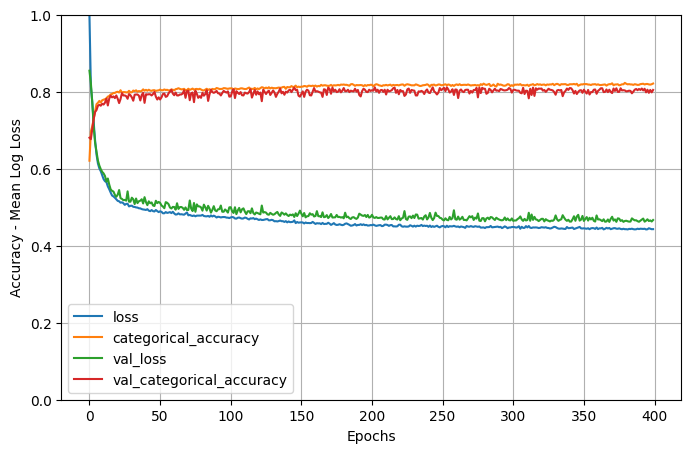
\includegraphics[scale=0.5]{d-tr-a2-e4.png}		
					\caption{Entrenamiento durante el Experimento 4 de la Arquitectura 2}	
					\label{d-tr-a2-e4}
				\end{center}
			\end{figure}
			
			Analizando la matriz de confusi\'on en la figura \ref{d-cm-a2-e4} vemos que ahora hemos solucionado el problema del modelo anterior que clasificaba todos los jugadores en la misma clase
			\begin{figure}[!h]
				\begin{center}
					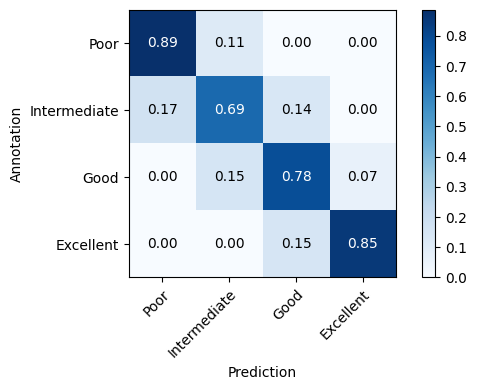
\includegraphics[scale=0.7]{d-cm-a2-e4.png}		
					\caption{Matriz de confusi\'on en el Experimento 4 de la Arquitectura 2}	
					\label{d-cm-a2-e4}
				\end{center}
			\end{figure}
		\newpage
		\subsubsection{Experimento 5: Reducimos \textit{batch-size}}
		\label{d-s-a2-e5}
			Decidimos reducir el \textit{batch size} para intentar reducir el \textit{bias} como en el experimento \ref{d-s-a1-e5}. La configuraci\'on para este experimento es:
			\begin{table}[!h]
				\begin{tabular}{| c | c | c | c | c | c | c |}
					\textbf{Epochs} & \textbf{Learning rate} & \textbf{Batch size} & \textbf{Activation} & \textbf{Loss} & \textbf{Optimizer} & \textbf{Regularization} \\ \hline
					400 & 0.001 & \textbf{64} & tanh & Categorical Crossentropy & ADAM & l2 0.001
				\end{tabular}
				\caption{Hiperpar\'ametros para el Experimento 5 de la Arquitectura 2}
				\label{tab:hip-d-a2-e5}
			\end{table}
			
			Tras 5 entrenamientos obtenemos los siguientes resultados:
			
			\begin{table}[!h]
				\begin{center}
					\begin{tabular}{ c | c | c | c | c | c |}
						\ & \textbf{Train accuracy (\%)} & \textbf{Validation accuracy (\%)} & \textbf{Bias (\%)} & \textbf{Variance (\%)} & \textbf{Training time (s)} \\ \hline
						\textbf{Mean} & 81.87 & 80.03 & 13.12 & 1.83 & 506.4 \\ \hline
						\textbf{Std} & 0.22 & 0.77 & 0.22 & 0.89 & 38.48 \\ \hline
					\end{tabular}
					\caption{Resultados del Experimento 5 de la Arquitectura 2}
					\label{tab:res-d-a2-e5}
				\end{center}
			\end{table}
			
			\begin{figure}[!h]
				\begin{center}
					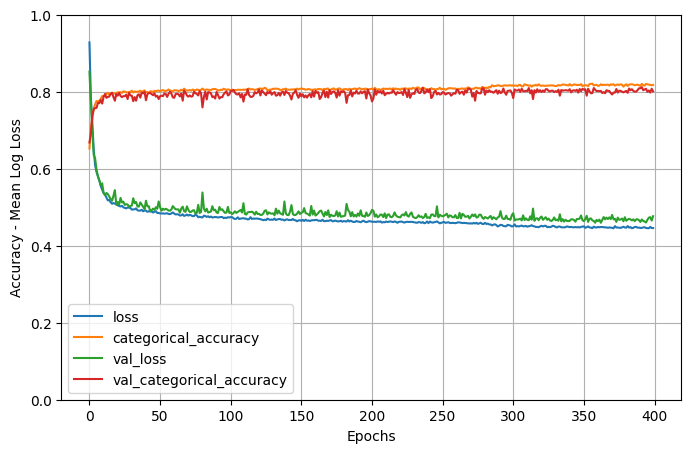
\includegraphics[scale=0.5]{d-tr-a2-e5.png}		
					\caption{Entrenamiento durante el Experimento 5 de la Arquitectura 2}	
					\label{d-tr-a2-e5}
				\end{center}
			\end{figure}
			
			\newpage
			No hemos obtenido mejora, este cambio no merece la pena porque aumenta mucho el tiempo de entrenamiento. Como vemos en la figura \ref{d-tr-a2-e5}, parece que el modelo deja de aprender, quiz\'as por el problema del \textit{vanishing gradient} que intentaremos resolver con la siguiente arquitectura.
		
		\subsubsection{Conclusiones de la Arquitectura 2}
		\label{d-cl-a2}
			A lo largo de estos experimentos hemos concluido que:
			\begin{itemize}
				\item La regularizaci\'on evita el \textit{overfitting}.
				\item El optimizador ADAM necesita un \textit{learning rate} bajo.
				\item El optimizador ADAM no ha proporcionado mejoras significativas con respecto al SGD para esta arquitectura.
			\end{itemize}
			
	\subsection{Arquitectura 3: Batch normalization}
	\label{d-s-a3}
		Despu\'es de no conseguir reducir el \textit{bias} de nuestro modelo con m\'as capas ocultas suponemos que estamos ante un problema de \textit{vanishing gradient}, una de las soluciones que existe es utilizar capas de \textit{batch normalization} para estandarizar los pesos de las neuronas. La arquitectura que utilizaremos durante los siguientes experimentos es:
		\begin{enumerate}
			\item Capa densa de 128 neuronas
			\item Capa de \textit{Batch Normalization} antes de la activaci\'on.
			\item Capa densa de 64 neuronas
			\item Capa de \textit{Batch Normalization} antes de la activaci\'on.
			\item Capa densa de 32 neuronas
			\item Capa de \textit{Batch Normalization} antes de la activaci\'on.
		\end{enumerate}
		
		\subsubsection{Experimento 1: Probamos la configuraci\'on del experimento \ref{d-s-a2-e5}}
		\label{d-s-a3-e1}
			Para comprobar como afecta la introducci\'on del \textit{batch normalization}, utilizamos la configuraci\'on del \'ultimo experimento realizado.
			
			\begin{table}[!h]
				\begin{tabular}{| c | c | c | c | c | c | c |}
					\textbf{Epochs} & \textbf{Learning rate} & \textbf{Batch size} & \textbf{Activation} & \textbf{Loss} & \textbf{Optimizer} & \textbf{Regularization} \\ \hline
					400 & 0.001 & 64 & tanh & Categorical Crossentropy & ADAM & l2 0.001
				\end{tabular}
				\caption{Hiperpar\'ametros para el Experimento 1 de la Arquitectura 3}
				\label{tab:hip-d-a3-e1}
			\end{table}
			
			Tras 5 entrenamientos obtenemos los siguientes resultados:
			
			\begin{table}[!h]
				\begin{center}
					\begin{tabular}{ c | c | c | c | c | c |}
						\ & \textbf{Train accuracy (\%)} & \textbf{Validation accuracy (\%)} & \textbf{Bias (\%)} & \textbf{Variance (\%)} & \textbf{Training time (s)} \\ \hline
						\textbf{Mean} & 89.23 & 76.23 & 5.76 & 15.59 & 950.4 \\ \hline
						\textbf{Std} & 0.46 & 1.54 & 0.46 & 1.75 & 55.11 \\ \hline
					\end{tabular}
					\caption{Resultados del Experimento 1 de la Arquitectura 3}
					\label{tab:res-d-a3-e1}
				\end{center}
			\end{table}
			La tabla \ref{tab:res-d-a3-e1} nos muestra que con \textit{batch normalization} hemos obtenido una buena \textit{accuracy} en el conjunto de entrenamiento pero a cambio de obtener un modelo con \textit{overfitting} como nos indica el \textit{variance} de 15\%. Tambi\'en ha sido la ejecuci\'on m\'as larga dado el tama\~no del batch y que hemos usado \textit{batch normalization} que ralentiza el proceso de entrenamiento.
			\newpage
			 
			\begin{figure}[!h]
				\begin{center}
					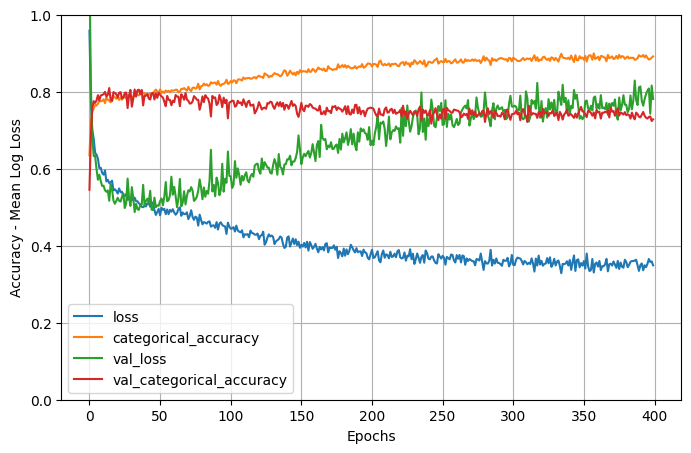
\includegraphics[scale=0.5]{d-tr-a3-e1.png}		
					\caption{Entrenamiento durante el Experimento 1 de la Arquitectura 3}	
					\label{d-tr-a3-e1}
				\end{center}
			\end{figure}
			
			En la figura \ref{d-tr-a3-e1} vemos como el modelo llega al punto de \textit{overfit} alrededor de la \textit{epoch} 50 donde el \textit{accuracy} de validaci\'on se separa del de entrenamiento.
			
		\subsubsection{Experimento 2: Aumentamos \textit{batch size}}
		\label{d-s-a3-e2}
			A\'un no hemos conseguido mejorar el \textit{accuracy} en el conjunto de validaci\'on, pero en este experimento vamos a intentar retrasar el \textit{overfitting} del modelo a la vez que el tiempo de entrenamiento aumentando el \textit{batch size}. La configuraci\'on para este experimento es la siguiente:
			\begin{table}[!h]
				\begin{tabular}{| c | c | c | c | c | c | c |}
					\textbf{Epochs} & \textbf{Learning rate} & \textbf{Batch size} & \textbf{Activation} & \textbf{Loss} & \textbf{Optimizer} & \textbf{Regularization} \\ \hline
					400 & 0.001 & \textbf{256} & tanh & Categorical Crossentropy & ADAM & l2 0.001
				\end{tabular}
				\caption{Hiperpar\'ametros para el Experimento 2 de la Arquitectura 3}
				\label{tab:hip-d-a3-e2}
			\end{table}
				
			Tras 5 entrenamientos obtenemos los siguientes resultados:
			\begin{table}[!h]
				\begin{center}
					\begin{tabular}{ c | c | c | c | c | c |}
						\ & \textbf{Train accuracy (\%)} & \textbf{Validation accuracy (\%)} & \textbf{Bias (\%)} & \textbf{Variance (\%)} & \textbf{Training time (s)} \\ \hline
						\textbf{Mean} & 97.02 & 73.89 & -2.02 & 23.17 & 254 \\ \hline
						\textbf{Std} & 0.53 & 0.48 & 0.53 & 0.61 & 14.04 \\ \hline
					\end{tabular}
					\caption{Resultados del Experimento 2 de la Arquitectura 3}
					\label{tab:res-d-a3-e2}
				\end{center}
			\end{table}
				
			\begin{figure}[!h]
				\begin{center}
					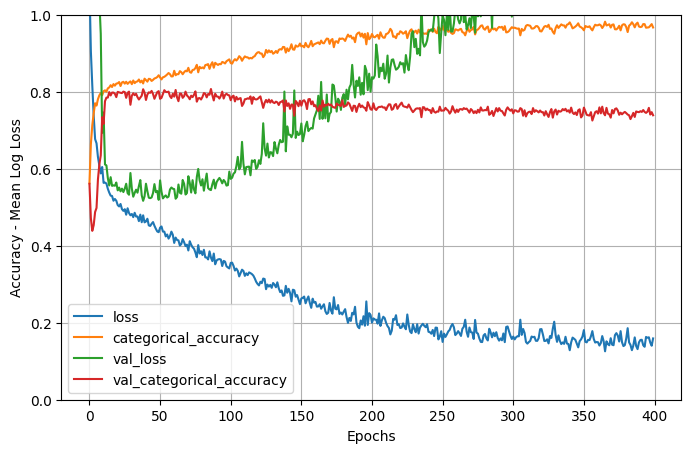
\includegraphics[scale=0.4]{d-tr-a3-e2.png}		
					\caption{Entrenamiento durante el Experimento 2 de la Arquitectura 3}	
					\label{d-tr-a3-e2}
				\end{center}
			\end{figure}
			Lo \'unico que hemos conseguido reducir con este experimento ha sido el tiempo de entrenamiento, el \textit{variance} ha aumentado hasta un 23\%.
			En la figura \ref{d-tr-a3-e2} vemos reflejado el \textit{overfitting}, lo que explica el \textit{bias} negativo.
			
		\subsubsection{Experimento 3: Aumentamos la penalizaci\'on del regularizador}
		\label{d-s-a3-e3}
			El regularizador L2 a\~nade una penalizaci\'on en base al tama\~no de los pesos, como no queremos que se descontrolen como ha estado ocurriendo, aumentamos esta penalizaci\'on para evitar el overfitting. La configuraci\'on para este experimento es:
			\begin{table}[!h]
				\begin{tabular}{| c | c | c | c | c | c | c |}
					\textbf{Epochs} & \textbf{Learning rate} & \textbf{Batch size} & \textbf{Activation} & \textbf{Loss} & \textbf{Optimizer} & \textbf{Regularization} \\ \hline
					400 & 0.001 & 256 & tanh & Categorical Crossentropy & ADAM & \textbf{l2 0.1}
				\end{tabular}
				\caption{Hiperpar\'ametros para el Experimento 3 de la Arquitectura 3}
				\label{tab:hip-d-a3-e3}
			\end{table}
			
			Tras 5 entrenamientos obtenemos los siguientes resultados:
			\begin{table}[!h]
				\begin{center}
					\begin{tabular}{ c | c | c | c | c | c |}
						\ & \textbf{Train accuracy (\%)} & \textbf{Validation accuracy (\%)} & \textbf{Bias (\%)} & \textbf{Variance (\%)} & \textbf{Training time (s)} \\ \hline
						\textbf{Mean} & 80.92 & 75.14 & 14.08 & 5.72 & 255.2 \\ \hline
						\textbf{Std} & 0.51 & 2.41 & 0.51 & 2.27 & 9.25 \\ \hline
					\end{tabular}
					\caption{Resultados del Experimento 3 de la Arquitectura 3}
					\label{tab:res-d-a3-e3}
				\end{center}
			\end{table}
			
			En este experimento hemos conseguido reducir considerablemente el \textit{variance} as\'i que podemos concluir que el aumento de la penalizaci\'on del regularizador sirve para evitar el \textit{overfitting}.
			\begin{figure}[!h]
				\begin{center}
					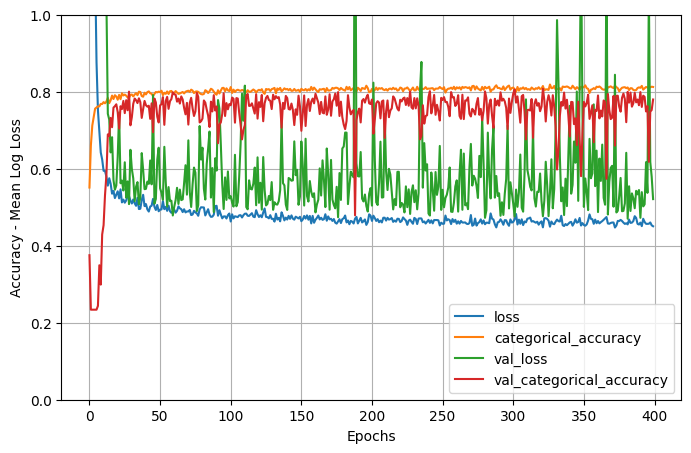
\includegraphics[scale=0.5]{d-tr-a3-e3.png}		
					\caption{Entrenamiento durante el Experimento 3 de la Arquitectura 3}	
					\label{d-tr-a3-e3}
				\end{center}
			\end{figure}
			En la figura \ref{d-tr-a3-e3} observamos una evoluci\'on err\'atica en el \textit{loss} en validaci\'on lo que puede indicar que el problema del \text{vanishing gradient} puede estar presente en el modelo.
			
		\subsubsection{Experimento 4: Volvemos a ReLU}
		\label{d-s-a3-e4}
			Cambiamos la funci\'on de activaci\'on a ReLU para comprobar si ayuda con el problema del \textit{vanishing gradient}.
			\begin{table}[!h]
				\begin{tabular}{| c | c | c | c | c | c | c |}
					\textbf{Epochs} & \textbf{Learning rate} & \textbf{Batch size} & \textbf{Activation} & \textbf{Loss} & \textbf{Optimizer} & \textbf{Regularization} \\ \hline
					400 & 0.001 & 256 & \textbf{ReLU} & Categorical Crossentropy & ADAM & l2 0.1
				\end{tabular}
				\caption{Hiperpar\'ametros para el Experimento 4 de la Arquitectura 3}
				\label{tab:hip-d-a3-e4}
			\end{table}
			\newpage			
			Tras 5 entrenamientos obtenemos los siguientes resultados:
			\begin{table}[!h]
				\begin{center}
					\begin{tabular}{ c | c | c | c | c | c |}
						\ & \textbf{Train accuracy (\%)} & \textbf{Validation accuracy (\%)} & \textbf{Bias (\%)} & \textbf{Variance (\%)} & \textbf{Training time (s)} \\ \hline
						\textbf{Mean} & 80.92 & 77.03 & 14.08 & 4.07 & 258.4 \\ \hline
						\textbf{Std} & 0.46 & 1.8 & 0.46 & 1.56 & 7.46 \\ \hline
					\end{tabular}
					\caption{Resultados del Experimento 4 de la Arquitectura 3}
					\label{tab:res-d-a3-e4}
				\end{center}
			\end{table}
			
			Hemos obtenido unos resultados similares al experimento anterior, adem\'as en la figura \ref{d-tr-a3-e4} se aprecia que no hay una fase de entrenamiento tan err\'atica.
			\begin{figure}[!h]
				\begin{center}
					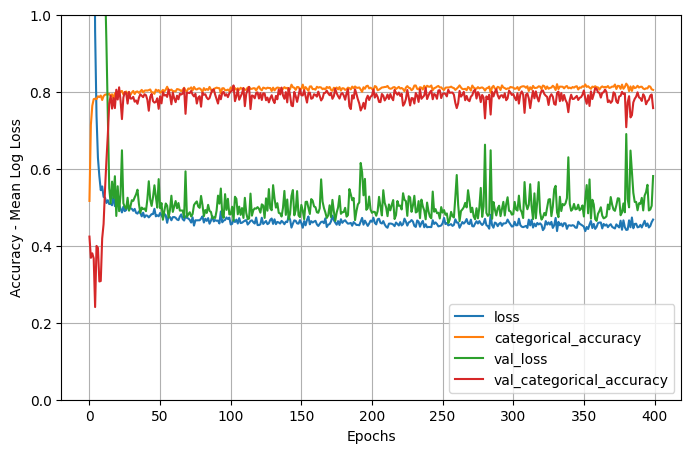
\includegraphics[scale=0.5]{d-tr-a3-e4.png}		
					\caption{Entrenamiento durante el Experimento 4 de la Arquitectura 3}	
					\label{d-tr-a3-e4}
				\end{center}
			\end{figure}
			
		\subsubsection{Experimento 5: Eliminamos la regularizaci\'on}
		\label{d-s-a3-e5}
			Nos preguntamos si tantos mecanismos contra el \textit{vanishing gradient} y \textit{overfitting} (\textit{batch normalization}, ReLU, regularizaci\'on L2) est\'an interfiriendo entre ellos as\'i que para comprobarlo retiramos la regularizaci\'on L2 de las capas ocultas.
			\begin{table}[!h]
				\begin{tabular}{| c | c | c | c | c | c | c |}
					\textbf{Epochs} & \textbf{Learning rate} & \textbf{Batch size} & \textbf{Activation} & \textbf{Loss} & \textbf{Optimizer} & \textbf{Regularization} \\ \hline
					400 & 0.001 & 256 & ReLU & Categorical Crossentropy & ADAM & \textbf{No}
				\end{tabular}
				\caption{Hiperpar\'ametros para el Experimento 5 de la Arquitectura 3}
				\label{tab:hip-d-a3-e5}
			\end{table}
			
			Tras 5 entrenamientos obtenemos los siguientes resultados:
			\begin{table}[!h]
				\begin{center}
					\begin{tabular}{ c | c | c | c | c | c |}
						\ & \textbf{Train accuracy (\%)} & \textbf{Validation accuracy (\%)} & \textbf{Bias (\%)} & \textbf{Variance (\%)} & \textbf{Training time (s)} \\ \hline
						\textbf{Mean} & 97.31 & 74.55 & -2.31 & 22.76 & 248 \\ \hline
						\textbf{Std} & 0.44 & 0.99 & 0.44 & 0.68 & 6.12 \\ \hline
					\end{tabular}
					\caption{Resultados del Experimento 5 de la Arquitectura 3}
					\label{tab:res-d-a3-e5}
				\end{center}
			\end{table}
			\newpage
			Definitivamente la regularizaci\'on es necesaria para evitar el \textit{overfitting}
			\begin{figure}[!h]
				\begin{center}
					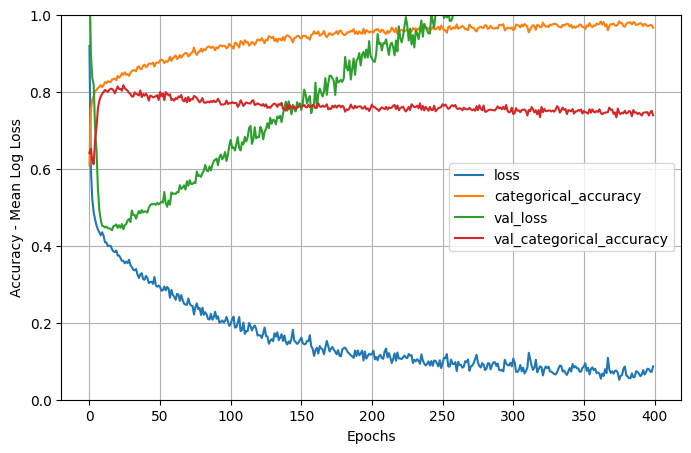
\includegraphics[scale=0.5]{d-tr-a3-e5.png}		
					\caption{Entrenamiento durante el Experimento 5 de la Arquitectura 3}	
					\label{d-tr-a3-e5}
				\end{center}
			\end{figure}
		
		\subsubsection{Conclusiones de la Arquitectura 3}
		\label{d-cl-a3}
			\begin{itemize}
				\item La regularizaci\'on L2 es necesaria para evitar el \textit{overfitting}.
				\item A mayor penalizaci\'on en L2 menor \textit{overfitting}.
				\item ReLU ayuda a mitigar el \textit{vanishing gradient}.
				\item Batch Normalization no ayuda a reducir el \textit{bias}.
			\end{itemize}
			
	\subsection{Arquitectura 4: A\~nadimos profundidad}
	\label{d-s-a4}
		Hasta el momento el m\'aximo \textit{accuracy} en validaci\'on que hemos conseguido ha sido en el experimento \ref{d-s-a1-e2} con un 81.5\%, nos parece que es un resultado malo para un problema de juguete como es este. Tras haber intentado distintos m\'etodos para reducir el \textit{bias} sin aumentar el \textit{variance} sin \'exito decidimos aumentar la profundidad de la red a 7 capas:
		\begin{enumerate}
			\item Capa densa de 2048 con Batch Normalization.
			\item Capa densa de 1048 con BN.
			\item Capa densa de 512 con BN.
			\item Capa densa de 256 con BN.
			\item Capa densa de 128 con BN.
			\item Capa densa de 64 con BN.
			\item Capa densa de 32 con BN.
		\end{enumerate}
		
		Cabe destacar que hemos estado repitiendo cada experimento 5 veces y no hemos encontrado diferencias significativas entre ellos, adem\'as una muestra aleatoria de tama\~no 5 no suele ser representativa del conjunto total. Creemos que el objetivo de esta pr\'actica es variar los hiperpar\'ametros y analizar su efecto en el modelo as\'i que a partir de este punto solo realizaremos cada experimento otra vez para poder probar m\'as combinaciones.
		\newpage
		
		\subsubsection{Experimento 1: Repetimos la \'ultima configuraci\'on}
		\label{d-s-a4-e1}
			Vamos a usar la configuraci\'on del experimento \ref{d-s-a3-e5} para comprobar como afecta el cambio de arquitectura.
			\begin{table}[!h]
				\begin{tabular}{| c | c | c | c | c | c | c |}
					\textbf{Epochs} & \textbf{Learning rate} & \textbf{Batch size} & \textbf{Activation} & \textbf{Loss} & \textbf{Optimizer} & \textbf{Regularization} \\ \hline
					400 & 0.001 & 256 & ReLU & Categorical Crossentropy & ADAM & No
				\end{tabular}
				\caption{Hiperpar\'ametros para el Experimento 1 de la Arquitectura 4}
				\label{tab:hip-d-a4-e1}
			\end{table}
			
			Y obtenemos los resultados:
			\begin{table}[!h]
				\begin{center}
					\begin{tabular}{| c | c | c | c | c |}
						\textbf{Train accuracy (\%)} & \textbf{Validation accuracy (\%)} & \textbf{Bias (\%)} & \textbf{Variance (\%)} & \textbf{Training time (s)} \\ \hline
						99.88 & 74.13 & -4.88 & 25.87 & 426 \\ \hline
					\end{tabular}
					\caption{Resultados del Experimento 1 de la Arquitectura 4}
					\label{tab:res-d-a4-e	}
				\end{center}
			\end{table}
			
			Como vemos hemos vuelto a obtener \textit{overfitting}, dado que no hemos reintroducido la regularizaci\'on desde el experimento \ref{d-s-a3-e5}.
			\begin{figure}[!h]
				\begin{center}
					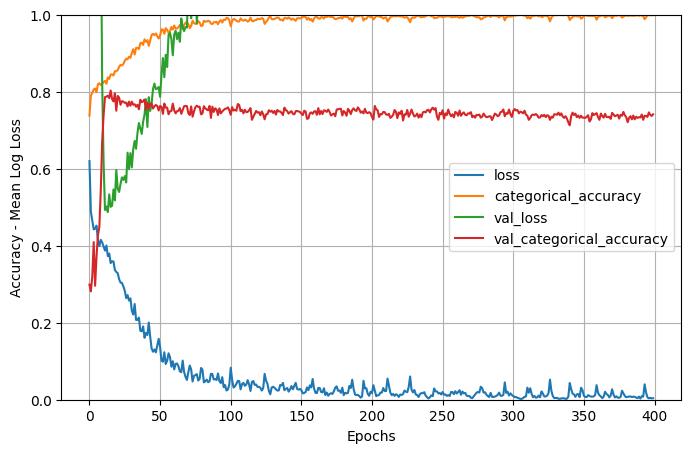
\includegraphics[scale=0.5]{d-tr-a4-e1.png}		
					\caption{Entrenamiento durante el Experimento 1 de la Arquitectura 4}	
					\label{d-tr-a4-e1}
				\end{center}
			\end{figure}
			
		\subsubsection{Experimento 2: Reintroducimos la regularizaci\'on L2}
		\label{d-s-a4-e2}
			Para evitar el \textit{overfitting} volvemos a usar la regularizaci\'on L2 con penalizaci\'on 0.1
			\begin{table}[!h]
				\begin{tabular}{| c | c | c | c | c | c | c |}
					\textbf{Epochs} & \textbf{Learning rate} & \textbf{Batch size} & \textbf{Activation} & \textbf{Loss} & \textbf{Optimizer} & \textbf{Regularization} \\ \hline
					400 & 0.001 & 256 & ReLU & Categorical Crossentropy & ADAM & \textbf{l2 0.1}
				\end{tabular}
				\caption{Hiperpar\'ametros para el Experimento 2 de la Arquitectura 4}
				\label{tab:hip-d-a4-e2}
			\end{table}
			
			Y obtenemos los resultados:
			\begin{table}[!h]
				\begin{center}
					\begin{tabular}{| c | c | c | c | c |}
						\textbf{Train accuracy (\%)} & \textbf{Validation accuracy (\%)} & \textbf{Bias (\%)} & \textbf{Variance (\%)} & \textbf{Training time (s)} \\ \hline
						80.99 & 74.75 & 14.01 & 6.24 & 457 \\ \hline
					\end{tabular}
					\caption{Resultados del Experimento 2 de la Arquitectura 4}
					\label{tab:res-d-a4-e2}
				\end{center}
			\end{table}
			
			Hemos evitado que el modelo haga \textit{overfitting} pero en la figura \ref{d-tr-a4-e2} se ve un entrenamiento demasiado err\'atico en cuanto al conjunto de validaci\'on, el \textit{loss} var\'ia enormemente en cada iteraci\'on, puede ser porque estemos estancados en un m\'inimo local.
			\begin{figure}[!h]
				\begin{center}
					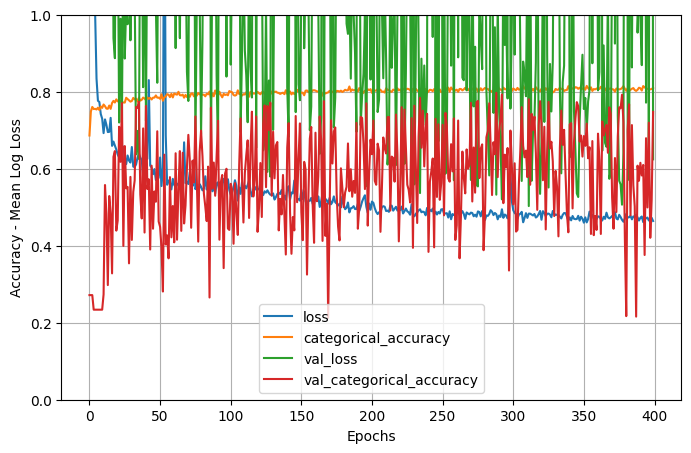
\includegraphics[scale=0.5]{d-tr-a4-e2.png}		
					\caption{Entrenamiento durante el Experimento 2 de la Arquitectura 4}	
					\label{d-tr-a4-e2}
				\end{center}
			\end{figure}
			
			En la matriz de confusi\'on, hemos detectado que por primera vez las clases "Intermediate" y "Good" son las que mayor \textit{recall} tienen lo que refuerza nuestra teor\'ia del m\'inimo local.
			\begin{figure}[!h]
				\begin{center}
					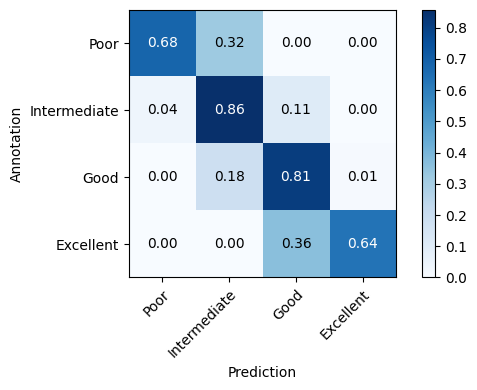
\includegraphics[scale=0.7]{d-cm-a4-e2.png}		
					\caption{Matriz de confusi\'on en el Experimento 2 de la Arquitectura 4}	
					\label{d-cm-a4-e2}
				\end{center}
			\end{figure}
			
		\subsubsection{Experimento 3: Desactivamos el bias de las capas ocultas}
		\label{d-s-a4-e3}
			En este momento reparamos en que estamos usando el vector \textit{bias} de las capas ocultas, pero no es necesario tenerlo en cuenta porque al estar usando \textit{Batch Normalization} ya estamos incluyendo un par\'ametro de \textit{offset} $\beta$. Vamos a comprobar si mejora el proceso de entrenamiento.
			
			\begin{table}[!h]
				\begin{tabular}{| c | c | c | c | c | c | c |}
					\textbf{Epochs} & \textbf{Learning rate} & \textbf{Batch size} & \textbf{Activation} & \textbf{Loss} & \textbf{Optimizer} & \textbf{Regularization} \\ \hline
					400 & 0.001 & 256 & ReLU & Categorical Crossentropy & ADAM & l2 0.1
				\end{tabular}
				\caption{Hiperpar\'ametros para el Experimento 3 de la Arquitectura 4}
				\label{tab:hip-d-a4-e3}
			\end{table}
			
			Y obtenemos los resultados:
			\begin{table}[!h]
				\begin{center}
					\begin{tabular}{| c | c | c | c | c |}
						\textbf{Train accuracy (\%)} & \textbf{Validation accuracy (\%)} & \textbf{Bias (\%)} & \textbf{Variance (\%)} & \textbf{Training time (s)} \\ \hline
						81.16 & 75.81 & 13.84 & 5.35 & 422 \\ \hline
					\end{tabular}
					\caption{Resultados del Experimento 3 de la Arquitectura 4}
					\label{tab:res-d-a4-e3}
				\end{center}
			\end{table}
			
			Como vemos, el cambio introducido no ha afectado al proceso de entrenamiento, simplemente hemos reducido el tiempo en 30 segundos.
			\begin{figure}[!h]
				\begin{center}
					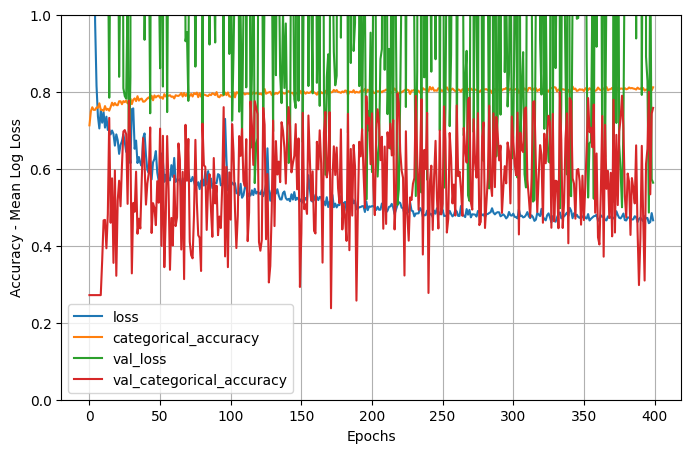
\includegraphics[scale=0.5]{d-tr-a4-e3.png}		
					\caption{Entrenamiento durante el Experimento 3 de la Arquitectura 4}	
					\label{d-tr-a4-e3}
				\end{center}
			\end{figure}
			
			En la matriz de confusi\'on comprobamos que la diagonal ha vuelto a los valores usuales.
			\begin{figure}[!h]
				\begin{center}
					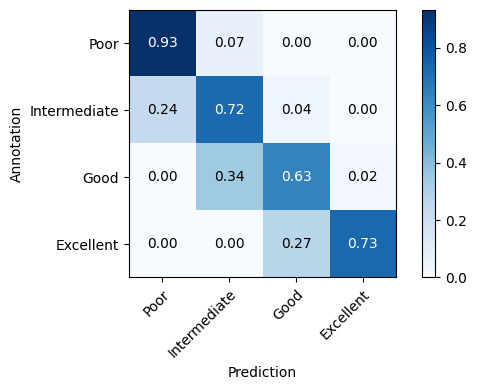
\includegraphics[scale=0.7]{d-cm-a4-e3.png}		
					\caption{Matriz de confusi\'on en el Experimento 3 de la Arquitectura 4}	
					\label{d-cm-a4-e3}
				\end{center}
			\end{figure}
			
			
		\subsubsection{Experimento 4: Usamos inicializadores}
        \label{s-a4-e4}
			Al estar usando una arquitectura profunda es importante que los pesos no se inicializen con valores demasiado altos ya que estos valores pueden crecer descontroladamente en las \'ultimas capas, as\'i que utilizaremos el initicializador \textit{He Normal}. La configuraci\'on queda as\'i:
			
			\begin{table}[!h]
				\begin{tabular}{|c|c|c|c|c|c|c|c|}
					\textbf{Epochs}&\textbf{Learning rate}&\textbf{Batch size}&\textbf{Activation}&\textbf{Loss}&\textbf{Optimizer}&\textbf{Regularization}  & \textbf{Initializer} \\ \hline
					400 & 0.001 & 256 & ReLU & C.C. & ADAM & l2 0.1 & \textbf{He Normal}
				\end{tabular}
				\caption{Hiperpar\'ametros para el Experimento 4 de la Arquitectura 4}
				\label{tab:hip-d-a4-e4}
			\end{table}
            \newpage
            			
			Y obtenemos los resultados:
			\begin{table}[!h]
				\begin{center}
					\begin{tabular}{| c | c | c | c | c |}
						\textbf{Train accuracy (\%)} & \textbf{Validation accuracy (\%)} & \textbf{Bias (\%)} & \textbf{Variance (\%)} & \textbf{Training time (s)} \\ \hline
						81.16 & 75.81 & 13.84 & 5.35 & 422 \\ \hline
					\end{tabular}
					\caption{Resultados del Experimento 4 de la Arquitectura 4}
					\label{tab:res-d-a4-e4}
				\end{center}
			\end{table}
			
			Como vemos, el cambio introducido no ha afectado al proceso de entrenamiento, simplemente hemos reducido el tiempo en 30 segundos. Puede que tengamos que cambiar el regularizador.
			\begin{figure}[!h]
				\begin{center}
					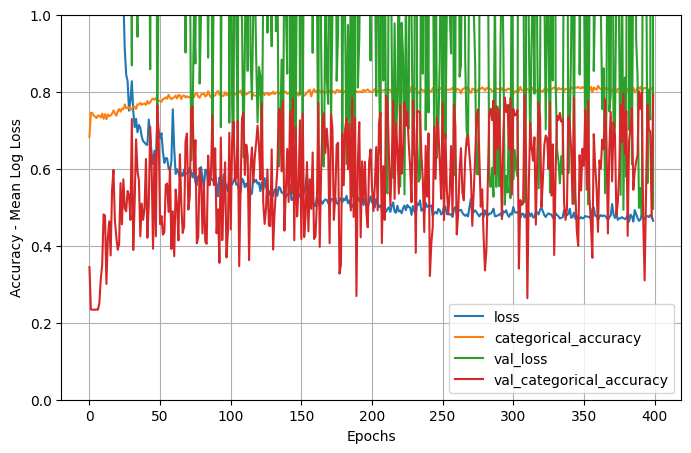
\includegraphics[scale=0.5]{d-tr-a4-e4.png}		
					\caption{Entrenamiento durante el Experimento 4 de la Arquitectura 4}	
					\label{tr-d-a4-e4}
				\end{center}
			\end{figure}
			
		\subsubsection{Experimento 5: Cambiamos el regularizador}
        \label{d-s-a4-e5}
			Creemos que el problema del entrenamient err\'atico est\'a producido por el regularizador, hemos aumentado mucho la penalizaci\'on y L2 a\~nade penalizaci\'on proporcional a la media del cuadrado de los pesos. Pensamos que utilizando L1 y reduciendo $\lambda$ conseguiremos solucionar nuestro problema.
			
			\begin{table}[!h]
				\begin{tabular}{|c|c|c|c|c|c|c|c|}
					\textbf{Epochs}&\textbf{Learning rate}&\textbf{Batch size}&\textbf{Activation}&\textbf{Loss}&\textbf{Optimizer}&\textbf{Regularization}  & \textbf{Initializer} \\ \hline
					400 & 0.001 & 256 & ReLU & C.C. & ADAM & \textbf{l1 0.0001} & He Normal
				\end{tabular}
				\caption{Hiperpar\'ametros para el Experimento 5 de la Arquitectura 4}
				\label{tab:hip-d-a4-e5}
			\end{table}
   
			Y obtenemos los resultados:
			\begin{table}[!h]
				\begin{center}
					\begin{tabular}{| c | c | c | c | c |}
						\textbf{Train accuracy (\%)} & \textbf{Validation accuracy (\%)} & \textbf{Bias (\%)} & \textbf{Variance (\%)} & \textbf{Training time (s)} \\ \hline
						95.86 & 74.01 & -0.86 & 21.85 & 455 \\ \hline
					\end{tabular}
					\caption{Resultados del Experimento 5 de la Arquitectura 4}
					\label{tab:res-d-a4-e5}
				\end{center}
			\end{table}

			Relajando la penalizaci\'on en la regularizaci\'on hemos vuelto al \textit{overfitting} como se ve en la tabla \ref{tab:res-d-a4-e5}, ya que tenemos un \textit{variance} de 22\%. Lo bueno es que hemos reducido la variaci\'on en el entrenamiento como vemos en la figura \ref{d-tr-a4-e5}.
			\begin{figure}[!h]
				\begin{center}
					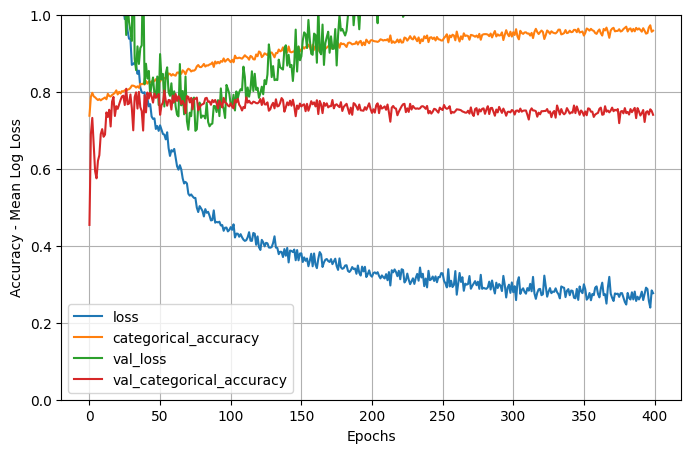
\includegraphics[scale=0.5]{d-tr-a4-e5.png}		
					\caption{Entrenamiento durante el Experimento 5 de la Arquitectura 4}	
					\label{d-tr-a4-e5}
				\end{center}
			\end{figure}
   
        \subsubsection{Experimento 6: Aumentamos \textit{batch size}}
        \label{d-s-a4-e6}
			Antes de pasar a la siguiente arquitectura decidimos aumentar el tama\~no del \textit{batch size} para probar si as\'i reducimos algo el \textit{overfitting}.
			
			\begin{table}[!h]
				\begin{tabular}{|c|c|c|c|c|c|c|c|}
					\textbf{Epochs}&\textbf{Learning rate}&\textbf{Batch size}&\textbf{Activation}&\textbf{Loss}&\textbf{Optimizer}&\textbf{Regularization}  & \textbf{Initializer} \\ \hline
					400 & 0.001 & \textbf{1024} & ReLU & C.C. & ADAM & l1 0.0001 & He Normal
				\end{tabular}
				\caption{Hiperpar\'ametros para el Experimento 6 de la Arquitectura 4}
				\label{tab:hip-d-a4-e6}
			\end{table}
            \newpage
			Y obtenemos los resultados:
			\begin{table}[!h]
				\begin{center}
					\begin{tabular}{| c | c | c | c | c |}
						\textbf{Train accuracy (\%)} & \textbf{Validation accuracy (\%)} & \textbf{Bias (\%)} & \textbf{Variance (\%)} & \textbf{Training time (s)} \\ \hline
						99.8 & 74.88 & -4.8 & 24.92 & 455 \\ \hline
					\end{tabular}
					\caption{Resultados del Experimento 6 de la Arquitectura 4}
					\label{tab:res-d-a4-e6}
				\end{center}
			\end{table}
   
			Ha aumentado el \textit{ovefitting}, de hecho el \textit{loss} del conjunto de validaci\'on no aparece en el gr\'afico de evoluci\'on durante el entrenamiento.
			\begin{figure}[!h]
				\begin{center}
					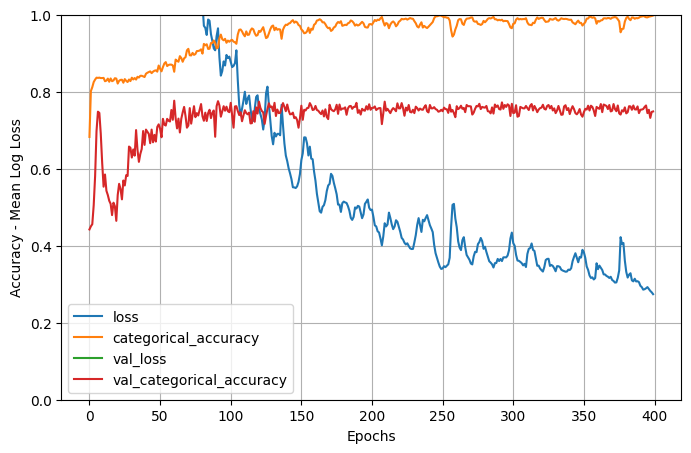
\includegraphics[scale=0.5]{d-tr-a4-e6.png}		
					\caption{Entrenamiento durante el Experimento 6 de la Arquitectura 4}	
					\label{d-tr-a4-e6}
				\end{center}
			\end{figure}
        \newpage
        
        \subsubsection{Experimento 7: Reducimos \textit{batch size}}
        \label{d-s-a4-e7}
			No estamos satisfechos con el \'ultimo experimento que adem\'as nos sugiere que a mayor \textit{batch size} mayor \textit{bias} por lo que lo reducimos a un tama\~no de 32.
			
			\begin{table}[!h]
				\begin{tabular}{|c|c|c|c|c|c|c|c|}
					\textbf{Epochs}&\textbf{Learning rate}&\textbf{Batch size}&\textbf{Activation}&\textbf{Loss}&\textbf{Optimizer}&\textbf{Regularization}  & \textbf{Initializer} \\ \hline
					400 & 0.001 & \textbf{32} & ReLU & C.C. & ADAM & l1 0.0001 & He Normal
				\end{tabular}
				\caption{Hiperpar\'ametros para el Experimento 7 de la Arquitectura 4}
				\label{tab:hip-d-a4-e7}
			\end{table}
			Y obtenemos los resultados:
			\begin{table}[!h]
				\begin{center}
					\begin{tabular}{| c | c | c | c | c |}
						\textbf{Train accuracy (\%)} & \textbf{Validation accuracy (\%)} & \textbf{Bias (\%)} & \textbf{Variance (\%)} & \textbf{Training time (s)} \\ \hline
						78.14 & 77.79 & 16.85 & 0.35 & 3239 \\ \hline
					\end{tabular}
					\caption{Resultados del Experimento 7 de la Arquitectura 4}
					\label{tab:res-d-a4-e7}
				\end{center}
			\end{table}
   
			Como vemos, reducir dr\'asticamente el \textit{batch size} ha eliminado por completo el \textit{overfitting} y de hecho el \textit{accuracy} del conjunto de entrenamiento y validaci\'on han convergido.
			\begin{figure}[!h]
				\begin{center}
					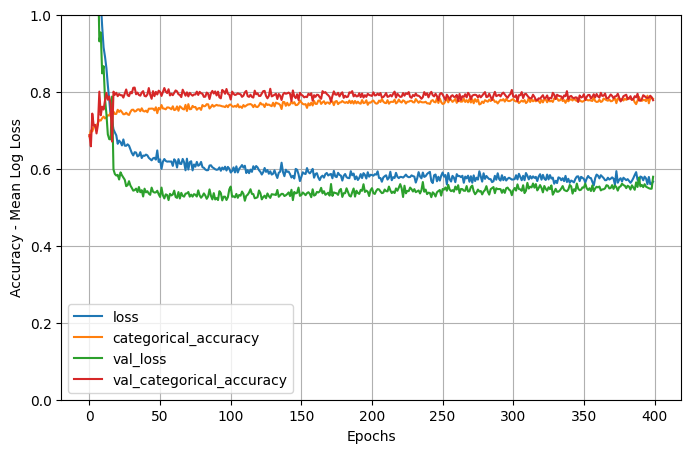
\includegraphics[scale=0.5]{d-tr-a4-e7.png}		
					\caption{Entrenamiento durante el Experimento 7 de la Arquitectura 4}	
					\label{d-tr-a4-e7}
				\end{center}
			\end{figure}
        \subsubsection{Conclusiones Arquitectura 4}
        \label{d-cl-a4}
            \begin{itemize}
                \item Sin regularizaci\'on el \textit{overfitting} persiste.
                \item A menor tama\~no del \textit{batch size} menor \textit{overfitting}.
                \item La regularizaci\'on L2 con un $\lambda$ grande hace que el entrenamiento sea err\'atico.
                \item Una arquitectura con mayor profundidad no ha producido una mejora en el \textit{bias}.
            \end{itemize}
            

    \subsection{Arquitectura 5: Arquitectura reloj de arena}
	\label{d-s-a5}
		Aunque no llega a ser un encoder-decoder, decidimos usar una arquitectura algo distinta a las que hemos estado usando hasta el momento. La arquitectura es la siguiente:
		\begin{enumerate}
			\item Capa densa de 512 neuronas con \textit{Batch Normalization}
			\item Capa densa de 128 neuronas con \textit{BN}
			\item Capa densa de 32 neuronas con \textit{BN}
			\item Capa densa de 128 neuronas con \textit{BN}
			\item Capa densa de 512 neuronas con \textit{BN}
		\end{enumerate}
		
		\subsubsection{Experimento 1: Probamos con la misma configuraci\'on del experimento \ref{d-s-a4-e7}}
		\label{d-s-a5-e1}
			Aqu\'i describir el cambio que hemos hecho con respecto al experimento anterior.
		
			\begin{table}[!h]
				\begin{center}
					\begin{tabular}{| c | c | c | c | c | c | c | c |}
						\textbf{Epochs} & \textbf{Learning rate} & \textbf{Batch size} & \textbf{Activation} & \textbf{Loss} & \textbf{Optimizer} & \textbf{Regularization} & \textbf{Initializer}\\ \hline
						 400 & 0.001 & 32 & ReLU & C.C. & ADAM & l1 0.0001 & He Normal
					\end{tabular}
					\caption{Hiperpar\'ametros para el Experimento 1 de la Arquitectura 5}
					\label{tab:hip-d-a5-e1}
				\end{center}
			\end{table}
			
			Y obtenemos los siguientes resultados:
			\begin{table}[!h]
				\begin{center}
					\begin{tabular}{| c | c | c | c | c |}
						\textbf{Train accuracy (\%)} & \textbf{Validation accuracy (\%)} & \textbf{Bias (\%)} & \textbf{Variance (\%)} & \textbf{Training time (s)} \\ \hline
						80.81 & 76.74 & 14.19 & 4.07 & 3414\\ \hline
					\end{tabular}
					\caption{Resultados del Experimento 1 de la Arquitectura 5}
					\label{tab:res-d-a5-e1}
				\end{center}
			\end{table}
		    
		    Como vemos, el \textit{variance} ha aumentado un 4\% y en cuanto a \textit{accuracy} hemos mejorado un 2\% en el conjunto de entrenamiento aunque empeorado m\'inimamente en cuanto al de validaci\'on. Es interesante el efecto que ha tenido esta arquitectura en el proceso de entrenamiento, los \textit{accuracys} de los dos conjuntos se cruzan siendo el de validaci\'on el que comienza con un mejor valor.
		    
			\begin{figure}[!h]
				\begin{center}
					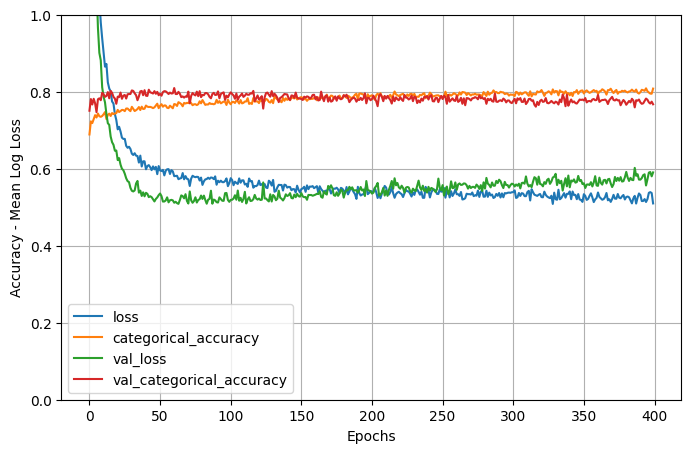
\includegraphics[scale=0.5]{d-tr-a5-e1.png}		
					\caption{Entrenamiento durante el Experimento 1 de la Arquitectura 5}	
					\label{d-tr-a5-e1}
				\end{center}
			\end{figure}
			Esta arquitectura no ha mejorado el \textit{bias} y en la matriz de confusi\'on mostrada en la figura \ref{d-cm-a5-e2} tampoco apreciamos cambios, las clases "Intermediate" y "Good" siguen siendo las clases con peor \textit{recall}.
			\begin{figure}[!h]
				\begin{center}
					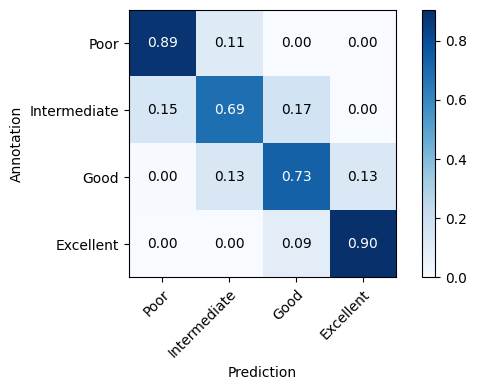
\includegraphics[scale=0.7]{d-cm-a5-e2.png}		
					\caption{Matriz de confusi\'on en el Experimento y de la Arquitectura x}	
					\label{d-cm-a5-e2}
				\end{center}
			\end{figure}
		
		\subsubsection{Experimento 2: Aumentamos \textit{batch size} y \textit{learning rate}}
		\label{d-s-a5-e2}
			El problema de tener un \textit{batch size} peque\~no es que el tiempo de entrenamiento aumenta de forma dr\'astica. En el paper \textit{Understanding Batch Normalization (2018)} de J. Bjorck et al. se menciona que el optimizador est\'a afectado por un ruido acotado superiormente por $\frac{lr}{bs}$, es decir por el \textit{learning rate} dividido por el \textit{batch size}. Esto implica que aumentar el \textit{batch size} tiene el mismo efecto que reducir el \textit{learning rate}. Como actualmente tenemos un buen equilibrio entre estos dos hiperpar\'ametros que no conduce al \textit{overfitting} vamos a aumentar ambos para mantener esta proporci\'on y adem\'as reducir el tiempo de entrenamiento.
		
			\begin{table}[!h]
				\begin{center}
					\begin{tabular}{| c | c | c | c | c | c | c | c |}
						\textbf{Epochs} & \textbf{Learning rate} & \textbf{Batch size} & \textbf{Activation} & \textbf{Loss} & \textbf{Optimizer} & \textbf{Regularization} & \textbf{Initializer}\\ \hline
						 400 & \textbf{0.01} & \textbf{256} & ReLU & C.C. & ADAM & l1 0.0001 & He Normal
					\end{tabular}
					\caption{Hiperpar\'ametros para el Experimento 2 de la Arquitectura 5}
					\label{tab:hip-d-a5-e2}
				\end{center}
			\end{table}
			\newpage
			Y obtenemos los siguientes resultados:
			\begin{table}[!h]
				\begin{center}
					\begin{tabular}{| c | c | c | c | c |}
						\textbf{Train accuracy (\%)} & \textbf{Validation accuracy (\%)} & \textbf{Bias (\%)} & \textbf{Variance (\%)} & \textbf{Training time (s)} \\ \hline
						84.43 & 80.21 & 10.57 & 4.22 & 379\\ \hline
					\end{tabular}
					\caption{Resultados del Experimento 2 de la Arquitectura 5}
					\label{tab:res-d-a5-e2}
				\end{center}
			\end{table}
		    
		    El efecto que hemos conseguido con este cambio ha sido muy satisfactorio, el tiempo de entrenamiento se ha reducido considerablemente y adem\'as hemos obtenido un mejor \textit{accuracy}. La pega es que con m\'as \textit{epochs} llegar\'iamos a un \textit{overfitting} como se aprecia en la figura \ref{d-tr-a5-e2}.
		    
			\begin{figure}[!h]
				\begin{center}
					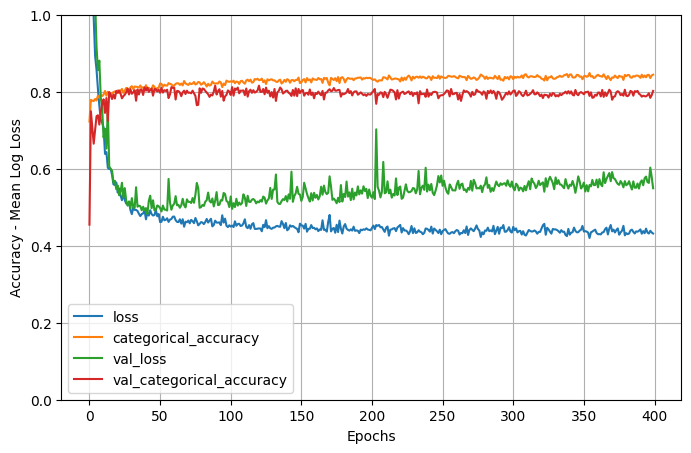
\includegraphics[scale=0.5]{d-tr-a5-e2.png}		
					\caption{Entrenamiento durante el Experimento 2 de la Arquitectura 5}	
					\label{d-tr-a5-e2}
				\end{center}
			\end{figure}
		
		\subsubsection{Experimento 3: Aumentamos \textit{batch size} y \textit{learning rate}}
		\label{d-s-a5-e3}
			Para evitar el problema del \textit{overfitting} a largo plazo que hemos detectado en el experimento \ref{d-s-a5-e2} introducimos una t\'ecnica que hasta ahora no hab\'iamos tenido en cuenta, el \textit{dropout}.
		
			\begin{table}[!h]
				\begin{center}
					\begin{tabular}{| c | c | c | c | c | c | c | c | c |}
						\textbf{Epochs} & \textbf{Learning rate} & \textbf{Batch size} & \textbf{Activation} & \textbf{Loss} & \textbf{Optimizer} & \textbf{Regularization} & \textbf{Initializer} & \textbf{Dropout}\\ \hline
						 400 & 0.01 & 256 & ReLU & C.C. & ADAM & l1 0.0001 & He Normal & \textbf{0.1}
					\end{tabular}
					\caption{Hiperpar\'ametros para el Experimento 3 de la Arquitectura 5}
					\label{tab:hip-d-a5-e3}
				\end{center}
			\end{table}
			Y obtenemos los siguientes resultados:
			\begin{table}[!h]
				\begin{center}
					\begin{tabular}{| c | c | c | c | c |}
						\textbf{Train accuracy (\%)} & \textbf{Validation accuracy (\%)} & \textbf{Bias (\%)} & \textbf{Variance (\%)} & \textbf{Training time (s)} \\ \hline
						80.13 & 75.37 & 14.87 & 4.76 & 382\\ \hline
					\end{tabular}
					\caption{Resultados del Experimento 3 de la Arquitectura 5}
					\label{tab:res-d-a5-e3}
				\end{center}
			\end{table}
		    
		    Hemos empeorado el \textit{bias} aunque hemos mantenido el \textit{variance} y como se ve en la figura \ref{d-tr-a5-e3} el entrenamiento se ha vuelto m\'as err\'atico aunque la divergencia que ve\'iamos entre los \textit{accuracy} de los conjuntos de entrenamiento y validaci\'on han desaparecido.
		    
			\begin{figure}[!h]
				\begin{center}
					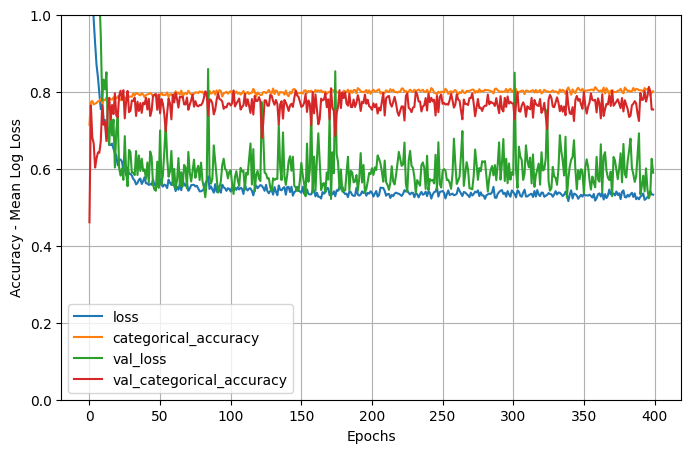
\includegraphics[scale=0.5]{d-tr-a5-e3.png}		
					\caption{Entrenamiento durante el Experimento 3 de la Arquitectura 5}	
					\label{d-tr-a5-e3}
				\end{center}
			\end{figure}
		
		
		\subsubsection{Experimento 4: Cambiamos la funci\'on de activaci\'on}
		\label{d-s-a5-e4}
			Otra opci\'on que no hemos probado hasta ahora es usar la funci\'on de activaci\'on \textit{eLU}, as\'i que en este experimento la usaremos con la esperanza de mejorar el \textit{bias} del modelo.
		
			\begin{table}[!h]
				\begin{center}
					\begin{tabular}{| c | c | c | c | c | c | c | c | c |}
						\textbf{Epochs} & \textbf{Learning rate} & \textbf{Batch size} & \textbf{Activation} & \textbf{Loss} & \textbf{Optimizer} & \textbf{Regularization} & \textbf{Initializer} & \textbf{Dropout}\\ \hline
						 400 & 0.01 & 256 & \textbf{eLU} & C.C. & ADAM & l1 0.0001 & He Normal & 0.1
					\end{tabular}
					\caption{Hiperpar\'ametros para el Experimento 4 de la Arquitectura 5}
					\label{tab:hip-d-a5-e4}
				\end{center}
			\end{table}
			\begin{table}[!h]
				\begin{center}
					\begin{tabular}{| c | c | c | c | c |}
						\textbf{Train accuracy (\%)} & \textbf{Validation accuracy (\%)} & \textbf{Bias (\%)} & \textbf{Variance (\%)} & \textbf{Training time (s)} \\ \hline
						80.25 & 77.67 & 14.75 & 2.58 & 388\\ \hline
					\end{tabular}
					\caption{Resultados del Experimento 4 de la Arquitectura 5}
					\label{tab:res-d-a5-e4}
				\end{center}
			\end{table}
		    
		    No hemos conseguido reducir el \textit{bias} pero si el \textit{variance} un 2\%. Como consecuencia de usar esta funci\'on de activaci\'on, el proceso de entrenamiento se ha visto afectado, la variaci\'on tanto en el \textit{loss} como en el \textit{accuracy} del conjunto de validaci\'on tiene una variaci\'on muy grande.
			\begin{figure}[!h]
				\begin{center}
					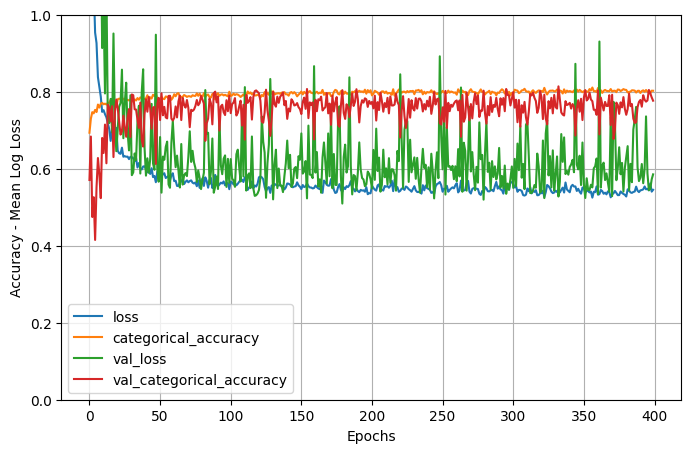
\includegraphics[scale=0.5]{d-tr-a5-e4.png}		
					\caption{Entrenamiento durante el Experimento 4 de la Arquitectura 5}	
					\label{d-tr-a5-e4}
				\end{center}
			\end{figure}
		
		
		\subsubsection{Conclusiones Arquitectura 5}
		\label{d-cl-a5}
			\begin{itemize}
				\item El \textit{dropout} consigue mitigar el \textit{overfitting}.
				\item La funci\'on de activaci\'on \textit{eLU} consigue un menor \textit{variance} en esta arquitectura.
			\end{itemize}
		
\section{Fase 2: Optimizaci\'on sistem\'atica}
	En esta fase iremos realizando cambios at\'omicos, es decir, para cada experimento nos centraremos en un hiperpar\'ametro a optimizar, qued\'andonos con el modelo que tenga mejor \textit{accuracy} en el conjunto de validaci\'on. Todos los experimentos a continuaci\'on han sido realizados 10 veces.
	\subsection{Arquitectura 1: MLP4}
			Probaremos una arquitectura de complejidad media para buscar el overfitting y aplicaremos t\'ecnicas de regularizaci\'on para reducir la varianza. 
			\begin{itemize}
			    \item Capa densa de 256 con Batch Normalization y Dropout = 0
                \item Capa densa de 124 con BN y Dropout = 0
                \item Capa densa de 64 con BN y Dropout = 0
                \item Capa densa de 32 con BN y Dropout = 0
			\end{itemize}
		\subsubsection{Experimento 1: Primera configuraci\'on}
        \label{s-a6-e1}
            Como se puede observar en la figura \ref{tab:tr-a6-e1}, tenemos un overfitting bastante grande y debemos aplicar t\'ecnicas de regularizaci\'on para mejorar la generalizaci\'on de la red. 
            \begin{table}[!h]
				\begin{tabular}{|c|c|c|c|c|c|c|c|c|}
					\textbf{Epochs}&\textbf{L.R}&\textbf{Batch size}&\textbf{Activation}&\textbf{Loss}&\textbf{Optimizer}&\textbf{Regularization}&\textbf{Dropout}   \\ \hline
					400 & 0.001 & 64 & ReLU & C.C. & ADAM & No & 0 
				\end{tabular}
				\caption{Hiperpar\'ametros para el Experimento 1 de la Arquitectura 6}
				\label{tab:hip-a6-e1}
			\end{table}
   
            \begin{table}[!h]
				\begin{center}
					\begin{tabular}{ c | c | c | c | c | c |}
						\ & \textbf{Train accuracy (\%)} & \textbf{Validation accuracy (\%)} & \textbf{Bias (\%)} & \textbf{Variance (\%)} & \textbf{Training time (s)} \\ \hline
						\textbf{Mean} & 98.7 & 70.47 & -3.7  & 28.23 & 817   \\ \hline
						\textbf{Std} &  0.83 & 0.28 &  0.83 & 0.86 & 8.4  \\ \hline
					\end{tabular}
					\caption{Resultados del Experimento 1 de la Arquitectura 6}
					\label{tab:res-a2-e5}
				\end{center}
			\end{table}
            
            \begin{figure}[!h]
				\begin{center}
					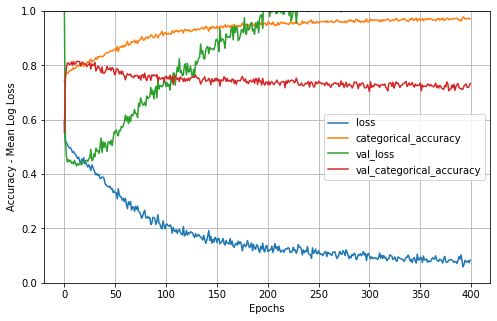
\includegraphics[scale=0.5]{tr-a6-e1.png}		
					\caption{Entrenamiento durante el Experimento 1 de la Arquitectura 6}	
					\label{tab:tr-a6-e1}
				\end{center}
			\end{figure}
   
        \subsubsection{Experimento 2: A\~{n}adimos Dropout 0.2}
        \label{s-a6-e2}
            Se a\~{n}ade un Dropout de 0.2 para reducir la varianza y mejorar la generalizaci\'on. La configuraci\'on es la siguiente: 
   
            \begin{table}[!h]
				\begin{tabular}{|c|c|c|c|c|c|c|c|c|}
					\textbf{Epochs}&\textbf{L.R}&\textbf{Batch size}&\textbf{Activation}&\textbf{Loss}&\textbf{Optimizer}&\textbf{Regularization}&\textbf{Dropout}   \\ \hline
					400 & 0.001 & 64 & ReLU & C.C. & ADAM & No & 0.2 
				\end{tabular}
				\caption{Hiperpar\'ametros para el Experimento 1 de la Arquitectura 6}
				\label{tab:hip-a6-e2}
			\end{table}
   
            Los resultados obtenidos son los siguientes: 
            \begin{table}[!h]
				\begin{center}
					\begin{tabular}{ c | c | c | c | c | c |}
						\ & \textbf{Train accuracy (\%)} & \textbf{Validation accuracy (\%)} & \textbf{Bias (\%)} & \textbf{Variance (\%)} & \textbf{Training time (s)} \\ \hline
						\textbf{Mean} & 88.28  & 76.67 & 6.72 & 11.61 & 743  \\ \hline
						\textbf{Std} & 1.15  & 0.79 & 1.15 & 1.89 & 8.9  \\ \hline
					\end{tabular}
					\caption{Resultados del Experimento 2 de la Arquitectura 6}
					\label{tab:res-a2-e5}
				\end{center}
			\end{table}
            \begin{figure}[!h]
				\begin{center}
					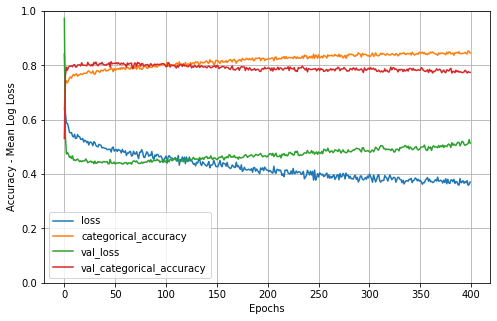
\includegraphics[scale=0.5]{tr-a6-e2.png}		
					\caption{Entrenamiento durante el Experimento 2 de la Arquitectura 6}	
					\label{tab:tr-a6-e2}
				\end{center}
			\end{figure}
            Se consigue una reducci\'on de la varianza a cambio de un empeoramiento del Bias. 
        
        \subsubsection{Experimento 3: Regularizac\'on L1, L2 y L1-L2 }
        Seguimos buscando la reducci\'on de la varianza. Para ello probaremos los regularizadores L1, L2 y L1-L2. 


      
        \begin{table}[!h]
				\begin{tabular}{|c|c|c|c|c|c|c|c|c|}
					\textbf{Epochs}&\textbf{L.R}&\textbf{Batch size}&\textbf{Activation}&\textbf{Loss}&\textbf{Optimizer}&\textbf{Regularization}&\textbf{Dropout}   \\ \hline
					400 & 0.001 & 64 & ReLU & C.C. & ADAM & ? & 0.2 
				\end{tabular}
				\caption{Hiperpar\'ametros para el Experimento 3 de la Arquitectura 6}
				\label{tab:hip-a6-e2}
			\end{table}

    
   
   \begin{table}[!h]
				\begin{center}
					\begin{tabular}{ c | c | c | c | c | c |}
						\ & \textbf{Train accuracy (\%)} & \textbf{Validation accuracy (\%)} & \textbf{Bias (\%)} & \textbf{Variance (\%)} & \textbf{Training time (s)} \\ \hline
						\textbf{L1 0.1} &63.6   &68.98  & 31.4  & -5.38 &  765 \\ \hline
						\textbf{L2 0.1} & 73.06   & 76.86 &  21.94 & -3.8 &864   \\ \hline
                        \textbf{L1-L2 0.1} &  63.7  &72.02 &  31.3 & -8.32 &804   \\ \hline
					\end{tabular}
					\caption{Resultados del Experimento 3 de la Arquitectura 6}
					\label{tab:res-a2-e5}
				\end{center}
			\end{table}
   
   \begin{figure}[!h]
				\begin{center}
					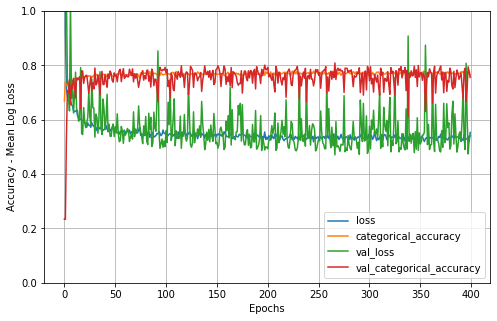
\includegraphics[scale=0.5]{tr-a6-e3.1.png}		
					\caption{Entrenamiento durante el Experimento 3 (L2) de la Arquitectura 6}	
					\label{tab:tr-a6-e2}
				\end{center}
			\end{figure}
    Como se puede observar la regularizac\'on L1 ha mejorado drasticamente la varianza y se ha conseguido una configuraci\'on que generaliza mejor. Sin embargo se ha aumentado demasiado el Bias, es por ello que en los siguientes experimentos habr\'a que intentar reducir el Bias. 
    
           La regularizac\'on L2 tambien ha conseguido reducir considerablemente la varianza, pero tiene la ventaja de que hemos conseguido menor empeoramiento que con L1. Se concluuye que en este caso es comveniente usar L2 frente a L1. En los siguientes experimentos habr\'a que intentar reducir el Bias, las soluciones partir\'ian de una reducci\'on del tama\~{n}o del Batch hasta una aumento de epochs. 
           
  La regularizaci\'on L1-L2 tambi\'en mejora dr\'asticamente la varianza, pero empeora en exceso el Bias. 

  Se concluye que el mejor regularizador para nuestra configuraci\'on actual es el L1. 
  
   

   
        \subsubsection{Experimento 4: Aumentar Epochs}
        En el experimento anterior se ha conseguido una mejora de la generalizaci\'on de la red a cambio de un alto Bias, es por ello que en este experimento se busca la reducci\'on del Bias utilizando m\'as epochs de entrenamiento. 
        
        \begin{table}[!h]
				\begin{tabular}{|c|c|c|c|c|c|c|c|c|}
					\textbf{Epochs}&\textbf{L.R}&\textbf{Batch size}&\textbf{Activation}&\textbf{Loss}&\textbf{Optimizer}&\textbf{Regularization}&\textbf{Dropout}   \\ \hline
					? & 0.001 & 64 & ReLU & C.C. & ADAM & L2 0.1 & 0.2 
				\end{tabular}
				\caption{Hiperpar\'ametros para el Experimento 3 de la Arquitectura 6}
				\label{tab:hip-a6-e2}
			\end{table}

    
   
   \begin{table}[!h]
				\begin{center}
					\begin{tabular}{ c | c | c | c | c | c |}
						 \textbf{epochs} & \textbf{Train accuracy (\%)} & \textbf{Validation accuracy (\%)} & \textbf{Bias (\%)} & \textbf{Variance (\%)} & \textbf{Training time (s)} \\ \hline
						\textbf{400 } & 73.06   & 76.86 &  21.94 & -3.8 &864   \\ \hline
                        \textbf{800 } & 73.52   &77.98 &  21.48 & -4.46  &1585    \\ \hline
                        \textbf{1200} &  72.64  &75.37  &  22.36& -2.73 &1944    \\ \hline
					\end{tabular}
					\caption{Resultados del Experimento 4 de la Arquitectura 6}
					\label{tab:res-a2-e5}
				\end{center}
			\end{table}

Duplicando o triplicando el n\'umero de epochs no se est\'a logrando una mejora significativa de la varianza. Esto puede ser debido a que la red se est\'a quedando atrapada en un m\'inimo local y hay que aplicar más reconfiguraciones para solventar este problema. 
\subsection{Experimento 5: Optimizadores}
Se van a probar los diferentes optimizadores con los hiper par\'ametros por defecto para buscar una mejor aproximaci\'on e intentar salir en el m\'inimo local en que se encuentra la red. 

 \begin{table}[!h]
				\begin{tabular}{|c|c|c|c|c|c|c|c|c|}
					\textbf{Epochs}&\textbf{L.R}&\textbf{Batch size}&\textbf{Activation}&\textbf{Loss}&\textbf{Optimizer}&\textbf{Regularization}&\textbf{Dropout}   \\ \hline
					800 & 0.001 & 64 & ReLU & C.C. & ? & L2 0.1 & 0.2 
				\end{tabular}
				\caption{Hiperpar\'ametros para el Experimento 5 de la Arquitectura 6}
				\label{tab:hip-a6-e2}
			\end{table}

    
   
   \begin{table}[!h]
				\begin{center}
					\begin{tabular}{ c | c | c | c | c | c |}
						 \textbf{Batch Size} & \textbf{Train accuracy (\%)} & \textbf{Validation accuracy (\%)} & \textbf{Bias (\%)} & \textbf{Variance (\%)} & \textbf{Training time (s)} \\ \hline
						\textbf{Adam } & 73.52   &77.98 &  21.48 & -4.46  &1585    \\ \hline
                        \textbf{RMSprop } & 71.39   &79.53  & 23.61  & -8.14  &  865   \\ \hline
                        \textbf{SGD} &  77.42   &  78.35& 17.58 & -0.93 &   683  \\ \hline
					\end{tabular}
					\caption{Resultados del Experimento 5 de la Arquitectura 6}
					\label{tab:res-a2-e5}
				\end{center}
			\end{table}
   
   \begin{figure}[!h]
				\begin{center}
					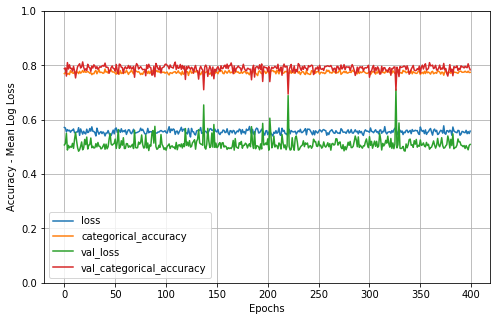
\includegraphics[scale=0.5]{Images/tr-a6-e5(SGD).png}		
					\caption{Entrenamiento durante el Experimento 5 (SGD) de la Arquitectura 6}	
					\label{tab:tr-a6-e2}
				\end{center}
			\end{figure}
   
   Como se puede observar con el optimizador SGD se consigue una liguera mejora en los resultados. Sin embargo, creemos que se puede conseguir mejores resultados ya que el Bias sigue siendo demasiado alto y la curva de aprendizaje es plana, lo que nos puede indicar que seguimos atrapados en un mínimo local. 
   \subsubsection{Experimento 6: Variando el Batch size}

Se sigue buscando una reducci\'on del Bias, para ello en este experimento se probar\'an diferentes tama\~{n}os de Batch para comprobar si se consigue una mejora. 

    \begin{table}[!h]
				\begin{tabular}{|c|c|c|c|c|c|c|c|c|}
					\textbf{Epochs}&\textbf{L.R}&\textbf{Batch size}&\textbf{Activation}&\textbf{Loss}&\textbf{Optimizer}&\textbf{Regularization}&\textbf{Dropout}   \\ \hline
					800 & 0.001 & ?& ReLU & C.C. & SGD & L2 0.1 & 0.2 
				\end{tabular}
				\caption{Hiperpar\'ametros para el Experimento 6 de la Arquitectura 6}
				\label{tab:hip-a6-e2}
			\end{table}

    
   
   \begin{table}[!h]
				\begin{center}
					\begin{tabular}{ c | c | c | c | c | c |}
						 \textbf{Optimizer} & \textbf{Train accuracy (\%)} & \textbf{Validation accuracy (\%)} & \textbf{Bias (\%)} & \textbf{Variance (\%)} & \textbf{Training time (s)} \\ \hline
	
                        \textbf{64} &  77.42   &  78.35& 17.58 & -0.93 &   683  \\ \hline
                        \textbf{32} &  73.9    & 79.16& 21.1 & -5.26 &   863  \\ \hline
                        \textbf{128} &  81.24  &  79.53& 13.76 &  1.71  &   443   \\ \hline
                        \textbf{256} &  84.74 &  78.47 & 10.26 & 6.27 &   383    \\ \hline
                        \textbf{1024} & 84.33 &  80.65 & 10.67 & 3.68 &   263     \\ \hline
                        \textbf{2048} & 75.45 &  79.34 & 19.55  & -3.89 &   323      \\ \hline
					\end{tabular}
					\caption{Resultados del Experimento 6 de la Arquitectura 6}
					\label{tab:res-a2-e5}
				\end{center}
			\end{table}
   El tama\~{n}o del batch \'optimo para la configuraci\'on actual es 1024. Obtenemos el mejor validation accuracy y Bias de los \'ultimos. Se concluye que al aumentar el tama\~{n}o del batch se consigue explorar m\'as y salir del m\'inimo local en el que nos encontr\'abamos antes. 

    \subsubsection{Experimento 7: Usando los nuevos datos}

En este experimento se probar\'a la mejor configuraci\'on con el nuevo dataset. Se observa que los resultados mejoran ligeramente, con lo cual se probar\'a a aumentar los epochs para comprobar si mejora el rendimiento. 

     \begin{table}[!h]
				\begin{tabular}{|c|c|c|c|c|c|c|c|c|}
					\textbf{Epochs}&\textbf{L.R}&\textbf{Batch size}&\textbf{Activation}&\textbf{Loss}&\textbf{Optimizer}&\textbf{Regularization}&\textbf{Dropout}   \\ \hline
					800 & 1024  & 64 & ReLU & C.C. & SGD & L2 0.1 & 0.2 
				\end{tabular}
				\caption{Hiperpar\'ametros para el Experimento 7 de la Arquitectura 6}
				\label{tab:hip-a6-e2}
			\end{table}
    
   
   \begin{table}[!h]
				\begin{center}
					\begin{tabular}{ c | c | c | c | c | c |}
						 \textbf{Epochs} & \textbf{Train accuracy (\%)} & \textbf{Validation accuracy (\%)} & \textbf{Bias (\%)} & \textbf{Variance (\%)} & \textbf{Training time (s)} \\ \hline
                        \textbf{800} & 81.51   & 82.45 & 13.49 & -0.94  &   383   \\ \hline
                        \textbf{1600} & 85.88   & 85.85 & 9.12 & 0.03  &  785    \\ \hline
                        \textbf{3000} & 88.61   & 85.72  & 6.39 & 2.89  &  1643     \\ \hline
                       
					\end{tabular}
					\caption{Resultados del Experimento 7 de la Arquitectura 6}
					\label{tab:res-a2-e5}
				\end{center}
			\end{table}

   El mejor modelo se obtiene con 1600 epochs, a partir de esos epochs sufrimos estancamiento en el validation accuracy, aunque se ha logrado una ligera mejora en el train accuracy. 	
	


	\section{Procesamiento de datos}
	\label{d-s-dp}
		En esta secci\'on comprobaremos c\'omo afecta en distintas arquitecturas el procesamiento de datos
		\subsection{Data imputation}
		\label{d-s-dp-di}
			Usando el notebook base de \textit{PreparingFootballPlayerDataset} lo modificamos para seleccionar distintas \textit{features} e imputar datos mediante \textbf{regresi\'on lineal} para el campo de \textit{Release Clause} e \textit{imputaci\'on de medias} para 48 jugadores con una puntuaci\'on global de 82.
			
		\subsection{Comparaci\'on de Arquitectura \ref{d-s-a1} con y sin data imputation}
		\label{d-s-dp-1}
			Usaremos la configuraci\'on del experimento \ref{d-s-a1-e2} y comparamos resultados:
			\begin{table}[!h]
				\begin{center}
					\begin{tabular}{ c | c | c | c | c | c |}
						\ & \textbf{Train accuracy (\%)} & \textbf{Validation accuracy (\%)} & \textbf{Bias (\%)} & \textbf{Variance (\%)} & \textbf{Training time (s)} \\ \hline
						\textbf{Sin DI} & 84.02 & 81.5 & 10.97 & 2.47 & 199\\ \hline
						\textbf{Con DI} & 85.52 & 83.31 & 9.48 & 2.21 & 180 \\ \hline
					\end{tabular}
					\caption{Comparaci\'on de resultados del Experimento 2 de la Arquitectura 1}
					\label{tab:res-d-a1-e2}
				\end{center}
			\end{table}
			
			\begin{figure}[!h]
				\centering
     			\begin{subfigure}[b]{0.4\textwidth}
         			\centering
         			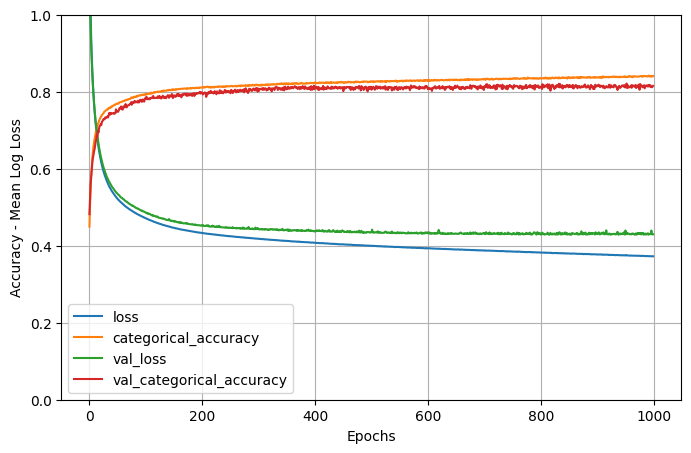
\includegraphics[scale=0.3]{d-tr-a1-e2}
         		\caption{Entrenamiento sin \textit{data imputation}}
         		\end{subfigure}
         		\hfill
     			\begin{subfigure}[b]{0.4\textwidth}
       				\centering
         			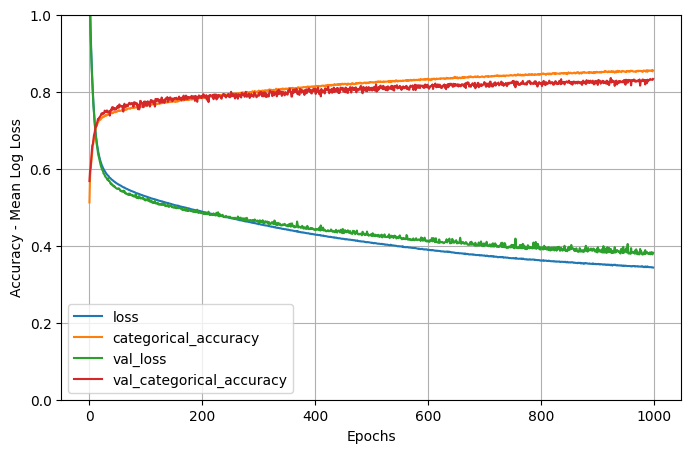
\includegraphics[scale=0.3]{d-tr-a1-e2-di}
         			\caption{Entrenamiento con \textit{data imputation}}
    		 	\end{subfigure}
    		 	\caption{Comparaci\'on del entrenamiento}
    		 	\label{d-s-tr-dp-1}
			\end{figure}
			La figura \ref{d-s-tr-dp-1} nos muestra la diferencia entre usar distintos datos en el entrenamiento. Con \textit{data imputation} obtenemos un entrenamiento en el que la red aprende de manera m\'as constante, adem\'as obtenemos mejores valores en todas las m\'etricas.
			
			\subsection{Comparaci\'on de Arquitectura \ref{d-s-a2} con y sin data imputation}
		\label{d-s-dp-2}
			Usaremos la configuraci\'on del experimento \ref{d-s-a3-e4} y comparamos resultados:
			\begin{table}[!h]
				\begin{center}
					\begin{tabular}{ c | c | c | c | c | c |}
						\ & \textbf{Train accuracy (\%)} & \textbf{Validation accuracy (\%)} & \textbf{Bias (\%)} & \textbf{Variance (\%)} & \textbf{Training time (s)} \\ \hline
						\textbf{Sin DI} & 80.92 & 77.03 & 14.08 & 4.07 & 258\\ \hline
						\textbf{Con DI} & 98.86 & 87.52 & -3.86 & 11.34 & 272 \\ \hline
					\end{tabular}
					\caption{Comparaci\'on de resultados del Experimento 4 de la Arquitectura 3}
					\label{tab:res-d-a1-e2}
				\end{center}
			\end{table}
			\begin{figure}[!h]
				\centering
     			\begin{subfigure}[b]{0.4\textwidth}
         			\centering
         			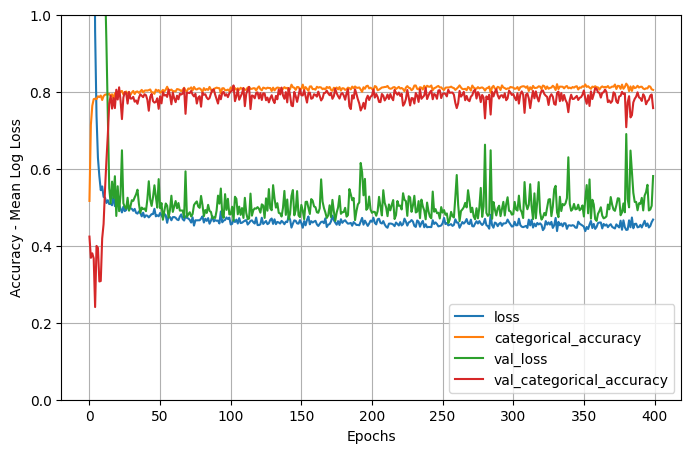
\includegraphics[scale=0.3]{d-tr-a3-e4}
         		\caption{Entrenamiento sin \textit{data imputation}}
         		\end{subfigure}
         		\hfill
     			\begin{subfigure}[b]{0.4\textwidth}
       				\centering
         			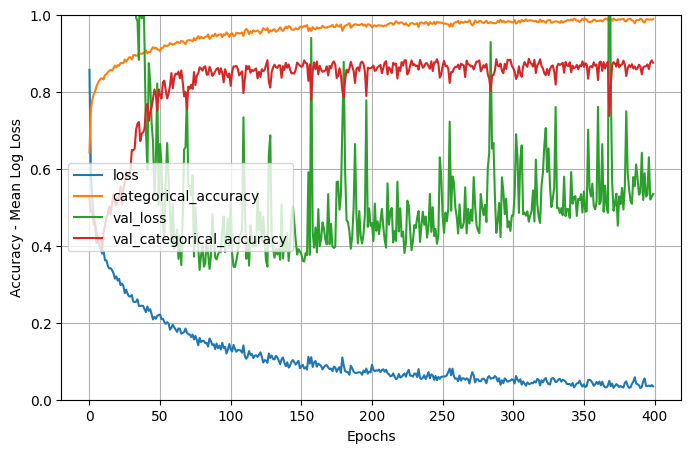
\includegraphics[scale=0.3]{d-tr-a3-e4-di}
         			\caption{Entrenamiento con \textit{data imputation}}
    		 	\end{subfigure}
    		 	\caption{Comparaci\'on del entrenamiento}
    		 	\label{d-s-tr-dp-2}
			\end{figure}
			La figura \ref{d-s-tr-dp-2} nos muestra la diferencia entre usar distintos datos en el entrenamiento. Con \textit{data imputation} obtenemos \textit{overfitting}, a\'un as\'i, el porcentaje de \textit{accuracy} en validaci\'on es el mayor obtenido hasta el momento y podemos asegurar que el procesamiento de los datos tiene un gran peso a la hora de mejorar resultados.
\end{document}
